
\documentclass{acmsiggraph}               % final
%\documentclass[review]{acmsiggraph}      % review
%\documentclass[widereview]{acmsiggraph}  % wide-spaced review
%\documentclass[preprint]{acmsiggraph}    % preprint

%% Uncomment one of the four lines above depending on where your paper is
%% in the conference process. ``review'' and ``widereview'' are for review
%% submission, ``preprint'' is for pre-publication, and ``final'' is for
%% the version to be printed.

%% These two line bring in essential packages: ``mathptmx'' for Type 1
%% typefaces, and ``graphicx'' for inclusion of EPS figures.

\usepackage{mathptmx}
\usepackage{graphicx}
\usepackage{epsfig}
\usepackage{amsmath,amscd,amssymb}

\newtheorem{theorem}{Theorem}[section]
\newtheorem{proposition}[theorem]{Proposition}
\newtheorem{definition}[theorem]{Definition}
\newtheorem{lemma}[theorem]{Lemma}
\newtheorem{corollary}[theorem]{Corollary}
\newtheorem{remark}[theorem]{Remark}


%% use this for zero \parindent and non-zero \parskip, intelligently.

\usepackage{parskip}

%% If you are submitting a paper to the annual conference, please replace
%% the value ``0'' below with your OnlineID. If you are not submitting this
%% paper to the annual conference, you may safely leave it at ``0'' -- it
%% will not be included in the output.

\onlineid{papers\_0142}

%% need to document this!

\acmformat{cameraready}

%% Paper title.

\title{Proposal: Visualizing the Loss Landscape of Neural Nets}

%% Author and Affiliation (single author).

%%\author{Roy G. Biv\thanks{e-mail: roy.g.biv@aol.com}\\Allied Widgets Research}

%% Author and Affiliation (multiple authors).

\author{Charles Ison\thanks{\small\texttt{e-mail: \{isonc|morgamat\}@eecs.oregonstate.edu}}\\ Oregon State University
\and Matthew Morgan$^{\ast}$ \\
Oregon State University}

%% Keywords that describe your work.

\keywords{rotational symmetry, field design, field analysis,
surfaces, topology, non-photorealistic rendering, remeshing.}

%%%%%% START OF THE PAPER %%%%%%

\begin{document}

\teaser{
%\centerline{\epsfig{file=images/teaser.eps,angle=0,width=\textwidth}}
    $\begin{array}{@{\hspace{-0.00in}}c@{\hspace{0.05in}}c@{\hspace{0.05in}}c@{\hspace{0.05in}}c}
    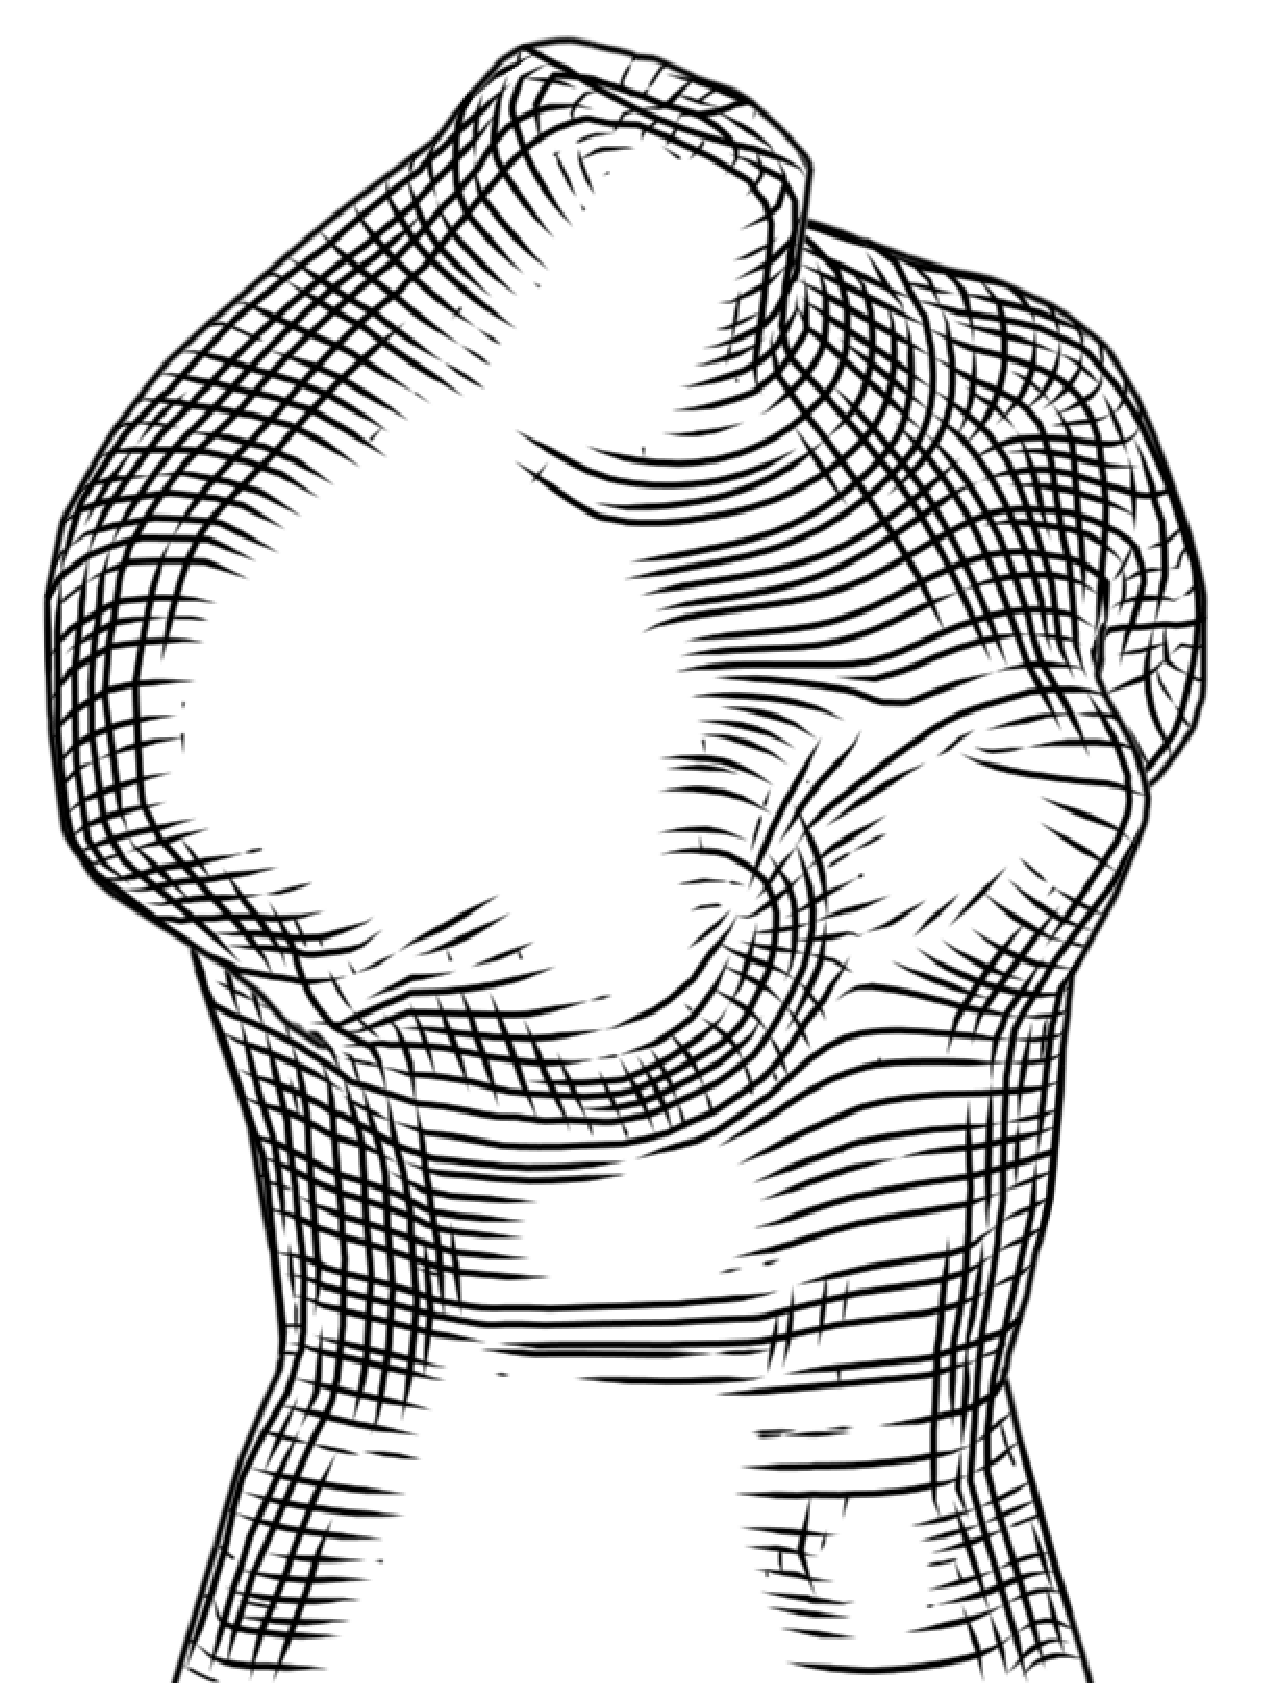
\includegraphics[width=1.75in]{images/venus_2sym_antiA.eps}
    &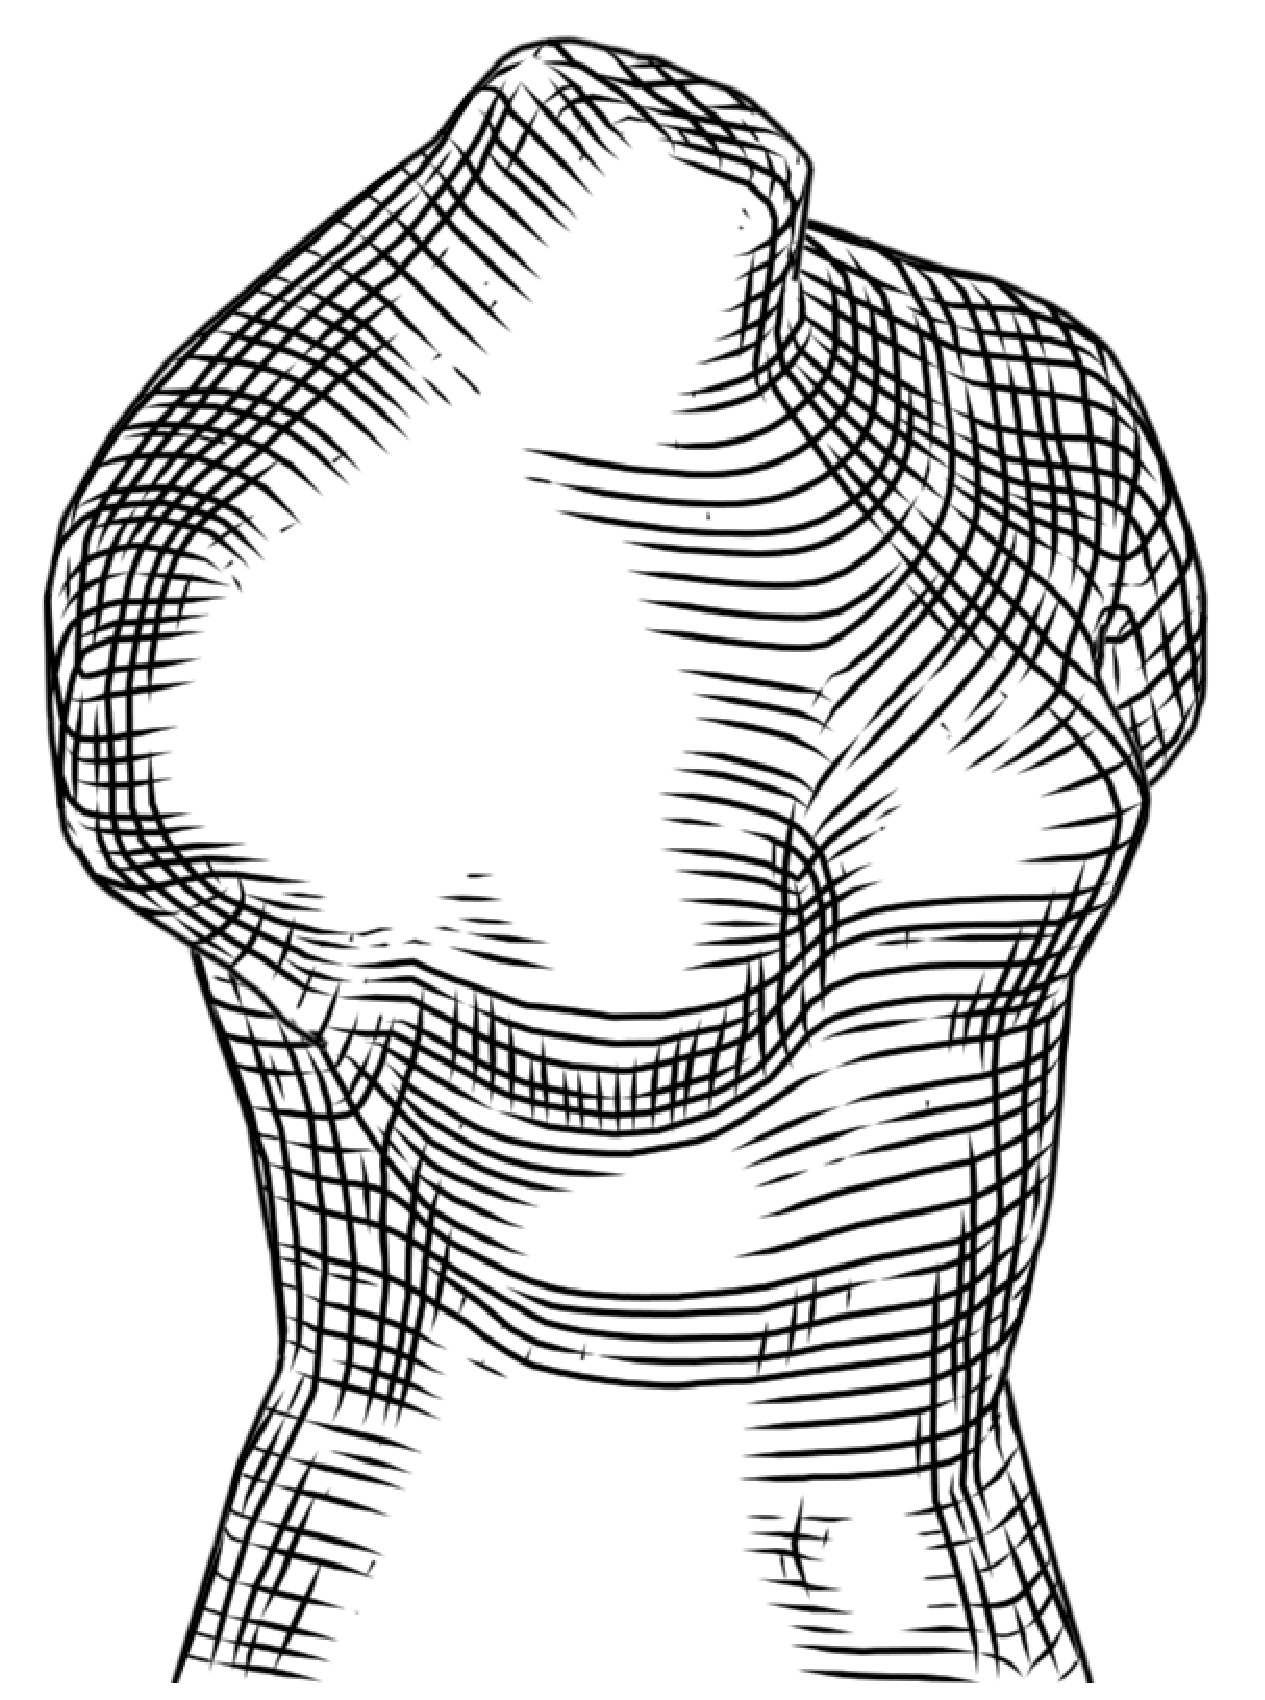
\includegraphics[width=1.75in]{images/venus_before_antiA.eps}
    &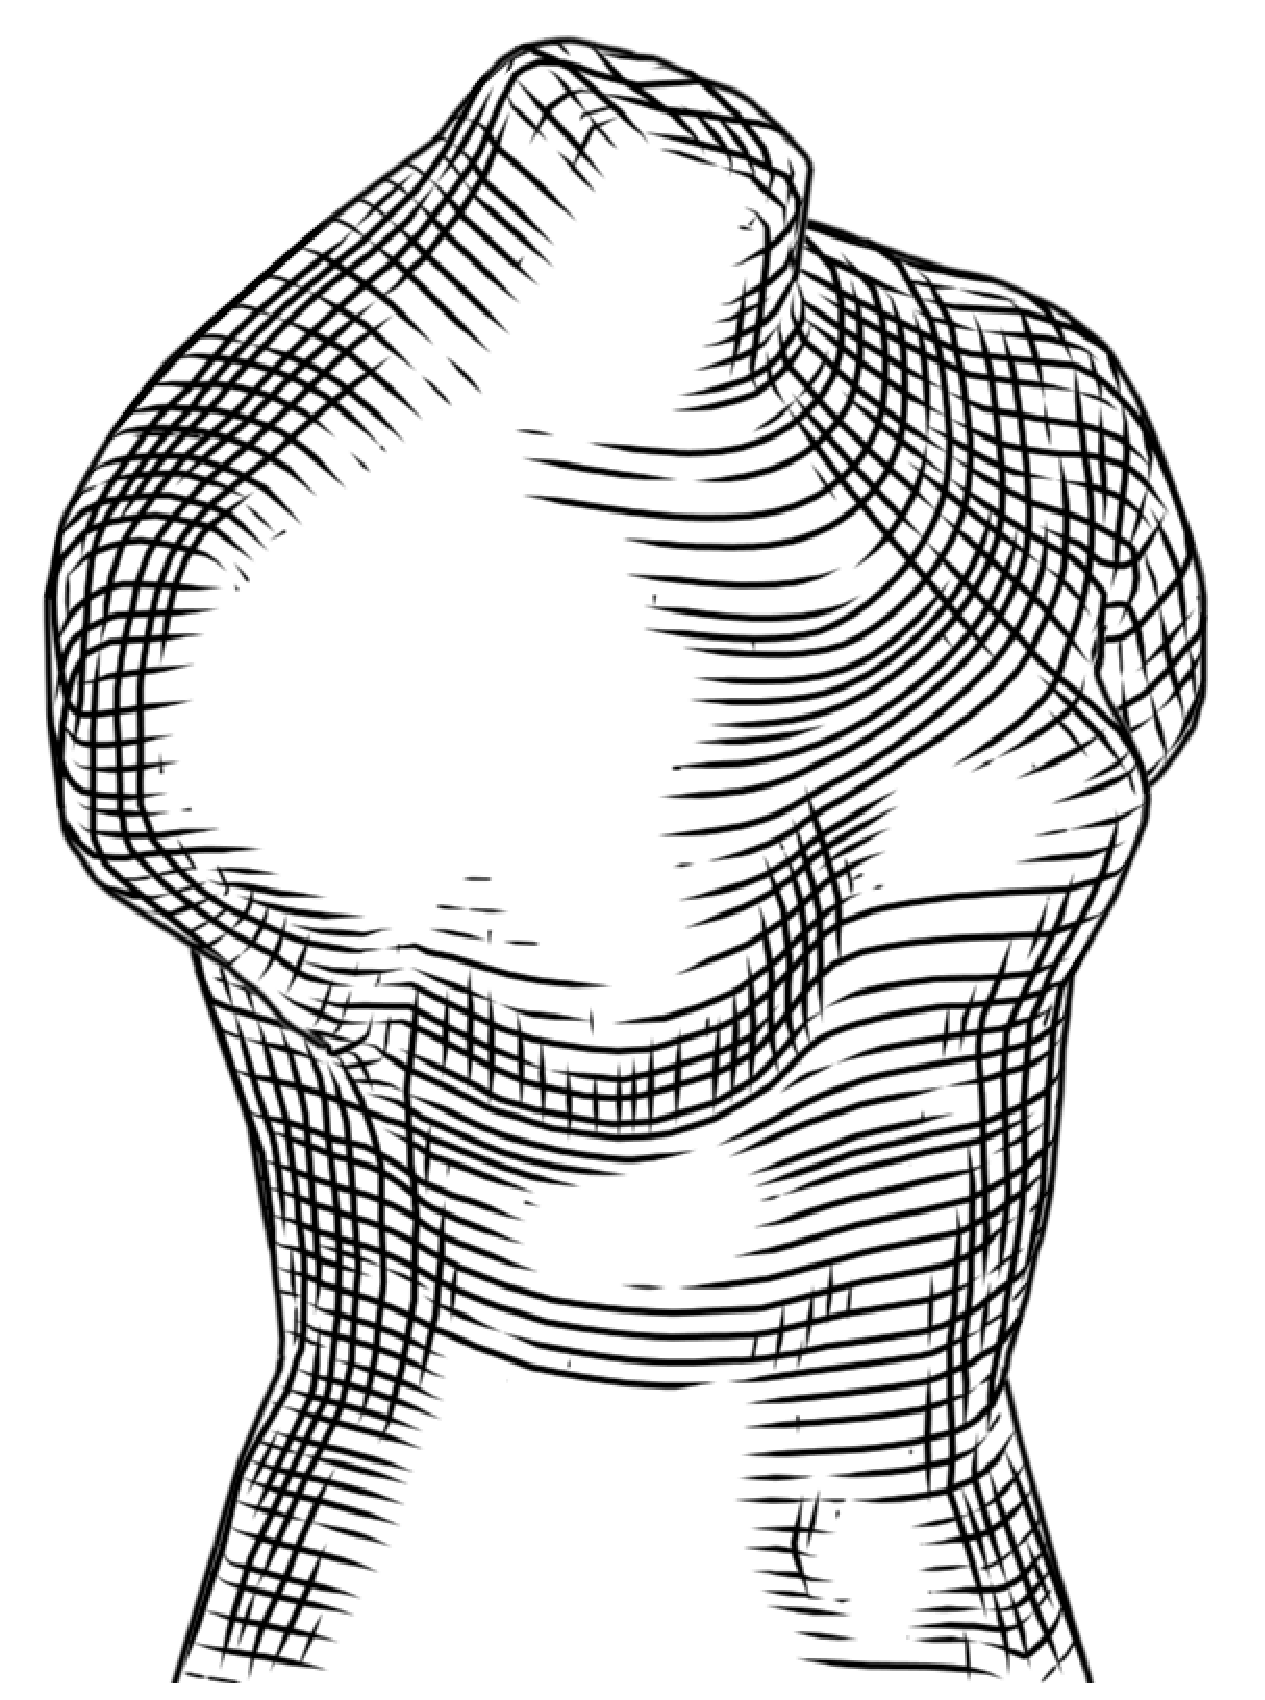
\includegraphics[width=1.75in]{images/venus_after_antiA.eps}
    &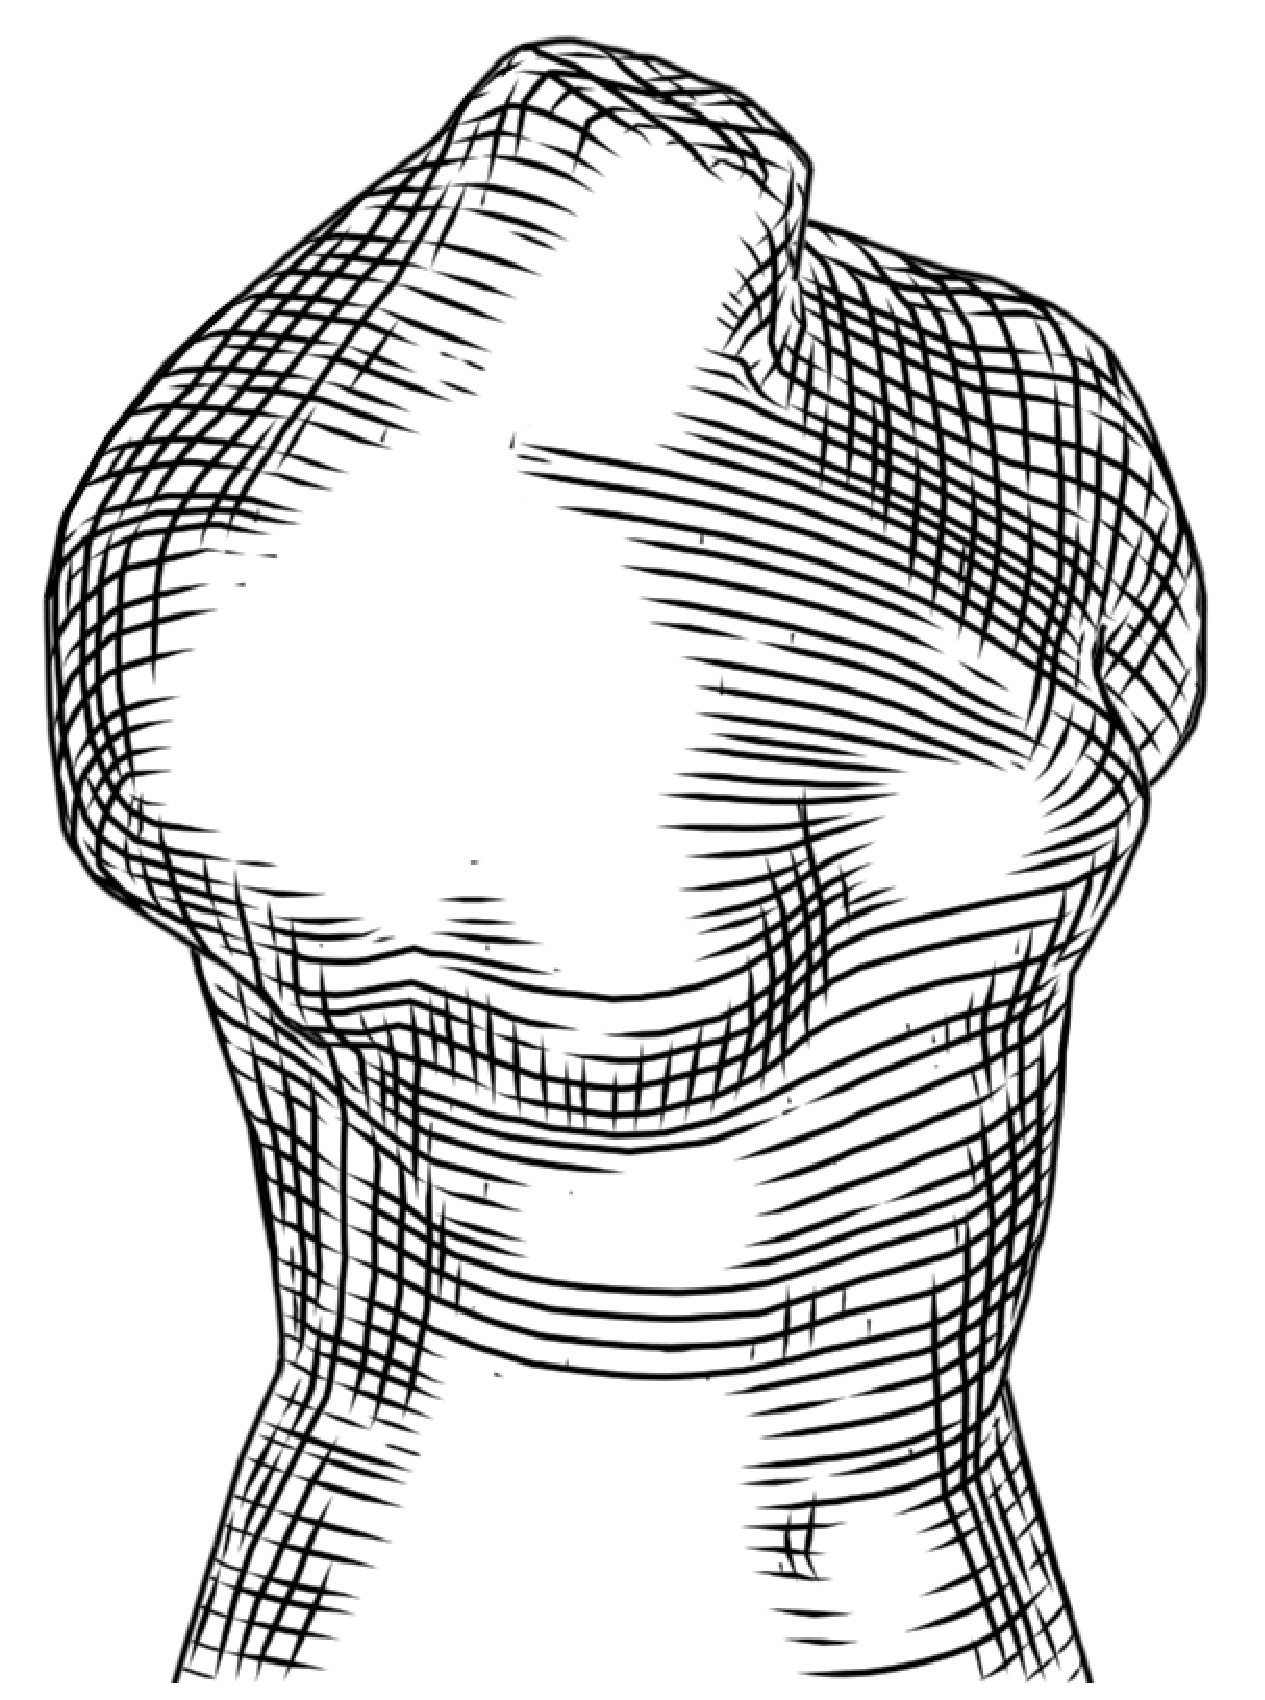
\includegraphics[width=1.75in]{images/venus_smooth_antiA.eps}\\
    (a)   &  (b)  & (c)  & (d)
    \end{array}$
\caption{Pen-and-ink sketching of the Venus using four different
fields: (a) the curvature tensor smoothed as a $2$-RoSy field, (b)
the curvature tensor smoothed as a $4$-RoSy field, (c) topological
editing operations applied to (b), and (d) more global smoothing
performed on (b). Notice that treating the curvature tensor as a
$4$-RoSy field (b) leads to fewer unnatural singularities and
therefore less visual artifacts than as a $2$-RoSy field (a). In
addition, both topological editing (c) and global smoothing (d) can
be used to remove more singularities from (b). However, topological
editing (c) provides local control while excessive global smoothing
(d) can cause hatch directions to deviate from their natural
orientations (neck and chest). } \label{fig:teaser} }

%% The ``\maketitle'' command must be the first command after the
%% ``\begin{document}'' command. It prepares and prints the title block.

\maketitle

%% Abstract section.

\begin{abstract}

\copyrightspace

Designing rotational symmetries on surfaces is a necessary task for
a wide variety of graphics applications, such as surface
parameterization and remeshing, painterly rendering and pen-and-ink
sketching, and texture synthesis. In these applications, the {\em
topology} of a rotational symmetry field such as {\em singularities}
and {\em separatrices} can have a direct impact on the quality of
the results. In this paper, we present a design system that provides
control over the topology of rotational symmetry fields on surfaces.

As the foundation of our system, we provide comprehensive analysis
for rotational symmetry fields on surfaces and present efficient
algorithms to identify singularities and separatrices. We also
describe design operations that allow a rotational symmetry field to
be created and modified in an intuitive fashion by using the idea of
basis fields and relaxation. In particular, we provide control over
the topology of a rotational symmetry field by allowing the user to
remove singularities from the field or to move them to more
desirable locations.

At the core of our analysis and design implementations is the
observation that $N$-way rotational symmetries can be described by
symmetric $N$-th order tensors, which allows an efficient
vector-based representation that not only supports coherent
definitions of arithmetic operations on rotational symmetries but
also enables many analysis and design operations for vector fields
to be adapted to rotational symmetry fields.

To demonstrate the effectiveness of our approach, we apply our
design system to pen-and-ink sketching and geometry remeshing.

\end{abstract}

%% ACM Computing Review (CR) categories.
%% See <http://www.acm.org/class/1998/> for details.
%% The ``\CRcat'' command takes four arguments.

\begin{CRcatlist}
  \CRcat{I.3.5}{Computer Graphics}{Computational Geometry and
Object Modeling}{Geometric algorithms, languages, and systems};
\end{CRcatlist}

%% The ``\keywordlist'' command prints out the keywords.
\keywordlist


\section{Introduction}
\label{sec:intro}


%% The ``\copyrightspace'' command must be the first command after the
%% start of the first section of the body of your paper. It ensures the
%% copyright space is left at the bottom of the first column on the first
%% page of your paper.


Many objects in computer graphics can be described by {\em
rotational symmetries}, such as brush strokes and hatches in
non-photorealistic rendering, regular patterns in texture synthesis,
and principle curvature directions in surface parameterization and
geometry remeshing. Intuitively, an {\em $N$-way rotational
symmetry} ($N$-RoSy) represents phenomena that are {\em invariant}
under rotations of an integer multiple of $\frac{2\pi}{N}$. Example
$N$-RoSy's include a vector ($N=1$), an eigenvector of a symmetric
matrix ($N=2$), and a cross ($N=4$). %Note we anticipate reflectional
%symmetries to be studied in the future, so we choose {\em RoSy} to
%distinguish.

\begin{figure*}[t]
\begin{center}
    $\begin{array}{@{\hspace{-0.00in}}c@{\hspace{0.05in}}c@{\hspace{0.05in}}c@{\hspace{0.05in}}c@{\hspace{0.05in}}c}
    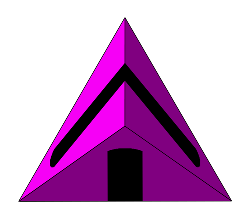
\includegraphics[height=1.3in]{images/tetra.eps}
    &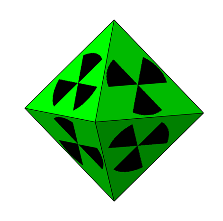
\includegraphics[height=1.3in]{images/octa.eps}
    &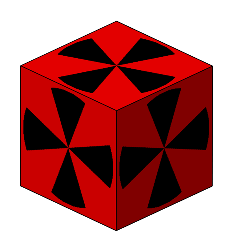
\includegraphics[height=1.3in]{images/cube.eps}
    &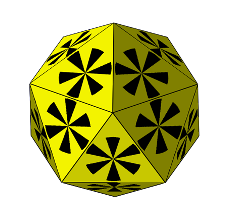
\includegraphics[height=1.3in]{images/icos.eps}
    &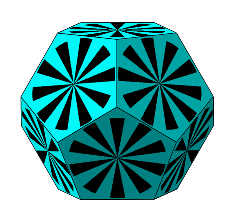
\includegraphics[height=1.3in]{images/dodec.eps}\\
    \end{array}$
\end{center}
\caption{$N$-way rotational symmetries appear naturally in the
Platonic solids: tetrahedron ($N=2$), octahedron ($N=3$), cube
($N=4$), icosahedron ($N=6$), and dodecahedron ($N=10$). }
\label{fig:symmetry_examples}
\end{figure*}

Symmetries naturally appear in surfaces, such as the five Platonic
shapes (Figure~\ref{fig:symmetry_examples}). Notice that the order
of the symmetry $N$ is equal to the ratio between $2\pi$ and the
angle of deficit at a vertex. In surfaces where global symmetry is
lacking, local symmetries can still occur, such as the singularities
(the vertices). In Figure~\ref{fig:teaser} (c), singularities of a
$4$-RoSy field appear in natural places such as the corner of the
shoulder (not visible due to the highlight) and under the armpit.

%\begin{figure*}[t]
%\begin{center}
%    $\begin{array}{@{\hspace{-0.00in}}c@{\hspace{0.05in}}c@{\hspace{0.05in}}c}
%    \includegraphics[width=2.3in]{images/issue2.eps}
%    &\includegraphics[width=2.3in]{images/issue3.eps}
%    &\includegraphics[width=2.3in]{images/issue4.eps}\\
%\end{array}$
%\end{center}
%\caption{ This figure illustrates the importance of a coherent
%representation of $N$-RoSy's with an example. Given the $3$-RoSy
%values defined at the vertices of triangle $\bigtriangleup{ABC}$,
%three methods were used to compute their average. In the left, one
%of the member vectors at $A$ was selected (magenta line) to decide
%the member vectors at $B$ and $C$ that has an angle of less than
%$\frac{\pi}{6}$ (magenta lines at $B$ and $C$). The average of three
%vectors (blue line at $O$) is considered to be a member vector of
%the $3$-RoSy at $O$ (the other two were colored in cyan). The same
%computational process is used for case shown in the middle with one
%exception: the first vertex where the member vector was chosen is
%$C$. This leads to a different member vector to be chosen at $B$,
%and the average of the member vectors is different from that of case
%in the left. Notice using the sum of member vectors lead to
%incoherent results. In contrast, the method used in the right is
%based on the {\em representation vectors} (yellow, see
%Section~\ref{sec:represent}) and therefore independent of the
%ambiguity in the member vectors.  }
%\label{fig:question}
%\end{figure*}

The ability to design and control $N$-RoSy fields on surfaces is
essential in many applications. For example, in non-photorealistic
rendering, the orientation of brush strokes and hatches are usually
guided by an $N$-RoSy field. Different artistic effects can be
achieved by using guiding fields with different characteristics. In
addition, singularities in the guiding field can lead to visual
artifacts such as brush strokes and hatches with unnatural
orientations. Singularities also present difficulties in the
construction of a global surface parameterization, where a
significant amount of stretch can occur in nearby regions.
Similarly, it is difficult to produce ideal triangular and quad
elements near singularities in geometry remeshing. For these
applications, a design system can be used to create a wide variety
of $N$-RoSy fields on surfaces, to add desirable features in an
existing field, and to control the number and location of the
singularities in the field. Most existing design systems focus on
vectors
($N=1$)~\cite{Praun:00,Turk:01,Wei:01,Theisel:02,Stam:03,Zhang:06}
and tensors ($N=2$)~\cite{Zhang:07}. A number of difficulties must
be addressed before a general design system can be developed for $N
\ge 3$.

First, there has been a lack of a mathematical representation for
rotational symmetries, which is required to define algebraic
operations on $N$-RoSy's such as sums and scalar multiples as well
as important concepts of $N$-RoSy fields such as singularities,
continuity, and differentiability.
%One way to define the sum of two $N$-RoSy's $s_1$
%and $s_2$ is to find a vector in $s_1$, which is used to locate a
%vector in $s_2$ that has the minimum angular difference. The sum of
%two vectors is then defined to be a vector in $s_1 + s_2$. As
%illustrated in Figure~\ref{fig:question} (left and middle), this
%approach can lead to inconsistencies when interpolating among three
%$N$-RoSy, which is a common task.
We overcome this difficulty by embedding $N$-way rotational
symmetries in the space of $N$-th order tensors, which allows
algebraic operations to be carried over from $N$-th order tensors to
$N$-RoSy's. We further derive a vector-based representation of
rotational symmetries based on the embedding, which enables
efficient analysis of $N$-RoSy fields on surfaces as well as allows
vector field design functionalities to be adapted to $N$-RoSy
fields. Furthermore, the concepts of singularities, continuity, and
differentiability are well-defined.

Second, there is relatively little understanding of the topological
structure in an $N$-RoSy field. While the concepts of singularities
have been used before, a proper definition of separatrices is
missing when $N \ge 3$. To address this, we present efficient
algorithms on extracting the singularities and separatrices in a
field. In particular, we adopt the approach of Zhang et
al.~\shortcite{Zhang:06} that allows continuous $N$-RoSy fields to
be generated on mesh surfaces despite the discontinuity in the
surface normal.

%Third, a design system requires fast and high-quality visualizations
%of the underlying fields. However, an $N$-RoSy field when $N \ge 3$
%has the property that there is more than one streamline that pass
%through every regular point in the domain. This makes it much
%difficult to visualize than vector fields ($N=1$) and tensor fields
%($N=2$) for which the number of streamlines is one. We present an
%approach that is based the IBFV and IBFVS techniques of van
%Wijk~\shortcite{vanWijk:02,vanWijk:03} but instead of using one
%image, we use either $N$ or $2N$ images depending on $N$ is even or
%odd. We show this approach is fast and high-quality for the cases
%$N=2, 3, 4, 6$, which cover the applications of this paper.
%
With the above issues addressed, we present a design system for
$N$-RoSy fields on surfaces that not only allows a wide variety of
$N$-RoSy fields to be generated but also provides explicit control
over the number and location of the singularities in the field. The
main functionalities of our work is reminiscent of that for vector
field design~\cite{Zhang:06}. However, the implementations are
rather different. For instance, we can create an initial $N$-RoSy
field on a surface using relaxation techniques~\cite{Turk:01} which
do not require a global surface parameterization. This greatly
increases the interactivity of our system. We also reuse algorithms
for singularity pair cancellation and movement in vector fields
through the aforementioned vector-based representation.

We have applied our design system to graphics applications such as
pen-and-ink sketching and quad-dominant remeshing.

%\begin{figure}[t]
%\begin{center}
%    $\begin{array}{@{\hspace{-0.00in}}c@{\hspace{0.05in}}c}
%    \includegraphics[height=1.1in]{images/4_separatrices_pos.eps}
%    &\includegraphics[height=1.1in]{images/4_separatrices_neg.eps}
%    \\
%    \end{array}$
%\end{center}
%\caption{Rotational symmetries appear naturally in the Platonic
%solids: octahedron ($3$), cube ($4$), icosahedron ($6$), and
%dodecahedron ($10$).  } \label{fig:symmetry_examples}
%\end{figure}

In this paper, we make the following contributions.

\begin{enumerate}
%\itemsep 0pt
%\parskip -1pt
\item We provide coherent definitions for algebraic
operations on $N$-RoSy's by observing the link between $N$-RoSy's
and $N$-th order symmetric tensors. This link also enables the
definitions of analytic properties of $N$-RoSy fields such as
continuity, differentiability, and singularity.
\item We present a vector-based representation for $N$-RoSy's that
supports compact storage of discrete $N$-RoSy fields on mesh
surfaces and facilitates the analysis and design of $N$-RoSy fields.
\item We describe the topology of $N$-RoSy fields on surfaces
and provide efficient algorithms to extract singularities and
separatrices.
\item We develop a design system in which $N$-RoSy fields
can be interactively created and modified on surfaces. In
particular, our system provides explicit control over the number and
location of the singularities in the field. We demonstrate the
effectiveness of our system with pen-and-ink sketching of surfaces
and quad-dominant remeshing.
%\item We present a visualization technique that is fast and
%high-quality when $N=2$, $3$, $4$, and $6$.
\end{enumerate}

The remainder of the paper is organized as follows. We first review
related work on $N$-RoSy fields in Section~\ref{sec:previous_work}
and present our vector-based representation of $N$-RoSy's in
Section~\ref{sec:representation}. Next, we discuss the analysis and
design of $N$-RoSy fields in Sections~\ref{sec:analysis}
and~\ref{sec:design}, respectively. In
Section~\ref{sec:application}, we show the results of applying our
analysis and design system to pen-and-ink sketching and geometry
remeshing. Finally, we summarize our contributions and discuss some
possible future work in Section~\ref{sec:conclusion}.

\section{Previous Work}
\label{sec:previous_work}

There has been a significant amount of work in the analysis and
design of vector and tensor fields. In contrast, relatively little
is known about $N$-RoSy fields when $N \ge 3$.

{\bf $N$-RoSy Analysis and Design:} To the best of our knowledge,
Hertzmann and Zorin~\shortcite{Hertzmann:00} are the first to
propose that hatches should follow a cross field ($4$-RoSy). They
provide a smoothing operation on $4$-RoSy fields that is based on a
non-linear optimization. Ray et al.~\shortcite{Ray:06} construct a
periodic global parameterization that facilitates quad remeshing. At
the heart of their approach is the use of $4$-RoSy fields, which
allows more natural-shaped quads to be generated near singularities.
They also develop a framework that allows the optimization to be
performed on the sines and cosines of the parameterization, which
turns a non-linear optimization into a linear one. They later
provide the analysis of singularities on $N$-RoSy's by extending the
Poincar\'e-Hopf theorem as well as describe an algorithm in which a
field with a minimal number of singularities can be constructed
based on user-specified constraints and the Euler characteristic of
the underlying surface~\cite{ray:07}.

{\bf Vector and Tensor Field Design:} There have been a number of
vector field design systems for surfaces. Most of them are generated
for a particular graphics application such as texture
synthesis~\cite{Praun:00,Turk:01,Wei:01}, fluid
simulation~\cite{Stam:03}, and vector field
visualization~\cite{vanWijk:02,vanWijk:03}. These systems do not
address topological control in the field. Systems providing
topological control include~\cite{Theisel:02,Zhang:06}. The system
of Zhang et al. has also been extended to create periodic
orbits~\cite{Chen:07} and to design tensor fields~\cite{Zhang:07}.
Our system is also reminiscent of the vector field design system of
Zhang et al.~\shortcite{Zhang:06} in terms of the functionality.
However, the implementation is rather different.

{\bf Vector and Tensor Field Analysis:} There has been much work in
vector and tensor field analysis. To review all the work is beyond
the scope of this paper. Here we refer to the most relevant work.
Helman and Hesselink~\shortcite{Helman:91} propose vector field
visualization techniques based on topological analysis. Delmarcelle
and Hesselink provide analysis of second-order symmetric tensor
fields~\shortcite{Delmarcelle:94}.

%Cabral and Leedom present a texture-based visualization for vector
%fields, which they termed {\em LIC} (Line-integral
%convolution)~\cite{Cabral:93}. This technique is of high quality.
%Later, van Wijk~\shortcite{vanWijk:02,vanWijk:03} provides an
%image-based flow visualization technique (IBFV) that is of similar
%quality but much faster due to the use of graphics hardware. Zhang
%et al.~\shortcite{Zhang:07} extend IBFV to symmetric second-order
%tensor fields.

\section{Vector-Based Representation}
\label{sec:representation}

The analysis and design of $N$-RoSy fields require coherent
definitions of the following concepts: summation and scalar
multiplication of $N$-RoSy's as well as continuity, singularity, and
differentiability. However, it is not immediately clear how to
define these concepts in a consistent manner given that a non-zero
$N$-RoSy $s$ consists of $N$ directions. For convenience, we will
refer to these directions the {\em member vectors} of $s$. Consider
the case when $N=2$, i.e., lines that can be modeled by eigenvectors
of a symmetric matrix with a zero trace~\cite{Zhang:07}. Given two
$2$-RoSy's $s_1 = \{ \pm
\begin{pmatrix} 1 \\ 0 \end{pmatrix} \}$ and $s_2 = \{ \pm
\begin{pmatrix} 0 \\ 1 \end{pmatrix} \}$, defining $s_1+s_2$
as the sum of member vectors can lead to inconsistent results: (1) $
\{ \pm
\begin{pmatrix} 1 \\ 1 \end{pmatrix} \}$, or (2) $\{ \pm
\begin{pmatrix} \quad 1 \\ -1 \end{pmatrix} \}$. As demonstrated by Zhang
et al.~\shortcite{Zhang:07}, treating a line field as a vector field
results in discontinuities and inconsistencies. This is also true
for $N$-RoSy fields when $N \ge 3$.

%In this section, we describe a vector-based representation for
%$N$-RoSy's, which removes the directional ambiguity in the $N$
%vectors representing an $N$-RoSy. This representation enables
%coherent definitions of important concepts and operations on
%$N$-RoSy fields, such as summation, scalar multiplication,
%continuity, singularity, and differentiability. We justify this
%representation by pointing out the link between $N$-RoSy's and
%$N$-th order tensors (also known as rank-$N$ tensors) in the
%Appendix.
%
%To illustrate the difficulties associated with the directional
%ambiguity in an $N$-RoSy, we consider the case when $N=2$, i.e.,
%lines that can be modeled by eigenvectors of a symmetric matrix with
%a zero trace~\cite{Zhang:07}. Given two $2$-RoSy's $s_1 = \{ \pm
%\begin{pmatrix} 1 & 0 \end{pmatrix}^{\bf T} \}$ and $s_2 = \{ \pm
%\begin{pmatrix} 0 & 1 \end{pmatrix}^{\bf T} \}$, defining $s_1+s_2$ using
%the sums of one of the two directions in the $2$-RoSy's can lead to
%inconsistent results: (1) $ \{ \pm
%\begin{pmatrix} 1 & 1 \end{pmatrix}^{\bf T} \}$, and (2) $\{ \pm
%\begin{pmatrix} 1 & -1 \end{pmatrix}^{\bf T} \}$. As demonstrated by Zhang
%et al.~\shortcite{Zhang:07}, treating a line field as a vector field
%results in discontinuities and inconsistencies. This is also true
%for $N$-RoSy's when $N \ge 3$.

To overcome this problem, we describe a representation for
$N$-RoSy's that is free of directional ambiguity. For an $N$-RoSy

\begin{equation}
s=\{\begin{pmatrix} R\cos(\theta + \frac{2k\pi}{N}) \\ R\sin(\theta
+ \frac{2k\pi}{N})
\end{pmatrix} \mid 0 \le k \le N-1 \}
\end{equation}

\noindent where $R\ge 0$ is the strength of $s$ and $\theta$ is the
angular component of one of the member vectors, we define the {\em
representation vector} of $s$ as $\begin{pmatrix} R\cos N\theta \\
R\sin N\theta \end{pmatrix}$. Notice that the representation vector
is independent of the choice of member vectors since

\begin{equation}
N(\theta + \frac{2k\pi}{N}) \equiv N\theta \mod 2\pi
\end{equation}

\noindent for any integer $k$. Consequently, directional ambiguity
no longer exists under this representation. We will define a map
$\gamma$ which maps an $N$-RoSy $s$ to its representation vector
$\gamma(s)$. Given two $N$-RoSy's $s_1$ and $s_2$ and a real number
$\lambda$, we define

\begin{equation}
s_1+s_2 = \gamma^{-1}(\gamma(s_1)+\gamma(s_2)), \quad \lambda s_1 =
\gamma^{-1}(\lambda \gamma(s_1))
\end{equation}

\noindent These definitions are coherent as they do not rely on the
choice of member vectors, which allow us to define important
concepts on $N$-RoSy fields, such as continuity, singularity, and
differentiability in a consistent manner.

A representation vector and a member vector differ in how their
components change under a change of basis. Consider the case where
the transformation matrix from the new basis to the original basis
has the form $Q =
\begin{pmatrix} \cos\varphi & -\sin\varphi
\\ \sin\varphi & \quad \cos\varphi \end{pmatrix}$. While a member
vector $v$ will have the form $Qv$ under the new basis, a
representation vector $w$ will be of the form $Q'w$ where
$Q'=\begin{pmatrix} \cos N\varphi & -\sin N\varphi \\ \sin N\varphi
& \quad \cos N\varphi \end{pmatrix}$. Therefore, a representation
vector is not a vector since its components do not change like a
vector under changes of basis. In the Appendix, we show that
$N$-RoSy's can be represented by symmetric $N$-th order covariant
tensors of a special form and such tensors can be compactly
represented by a vector (representation vector) under any given
basis. Consequently, the components of a representation vector
transform differently than a vector under a change of basis.

As will become apparent soon, $\gamma$ not only provides a coherent
and compact representation of $N$-RoSy's, but also allows efficient
implementations of key operations on $N$-RoSy fields by borrowing
corresponding algorithms for vector fields, such as interpolations
and singularity extraction (Section~\ref{sec:represent}), blending
(Section~\ref{sec:initialization}), and topological editing
(Section~\ref{sec:edit}). Figure~\ref{fig:vector_representation}
shows a $4$-RoSy field (left) and its representation vector field
(right). Notice that they have the same set of singularities. Next,
we discuss the analysis and design of $N$-RoSy fields on surfaces.

\begin{figure}[t]
\begin{center}
    $\begin{array}{@{\hspace{-0.00in}}c@{\hspace{0.05in}}c}
    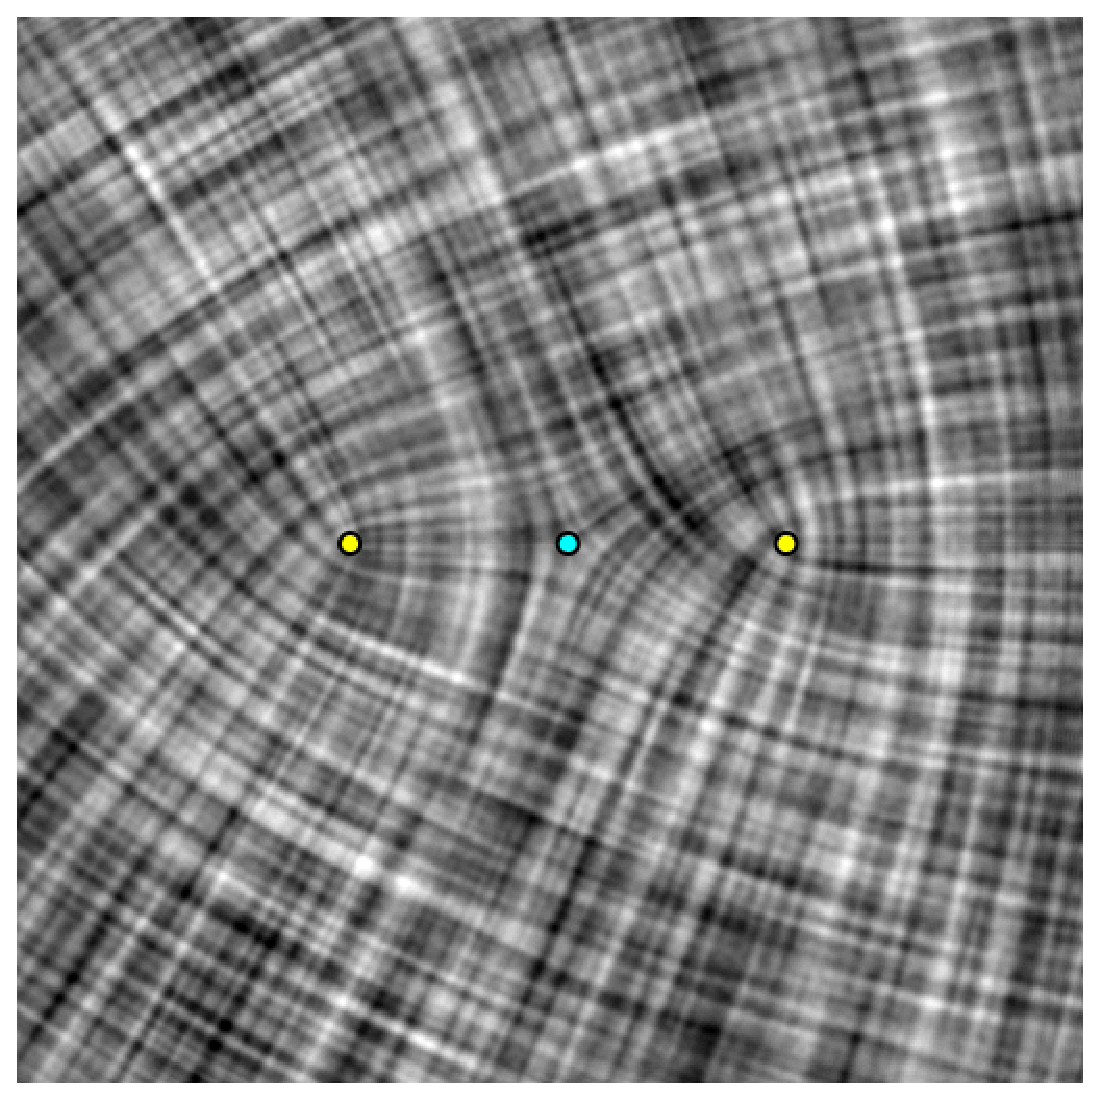
\includegraphics[height=1.07in]{images/cancel_step0_4sym.eps}
    &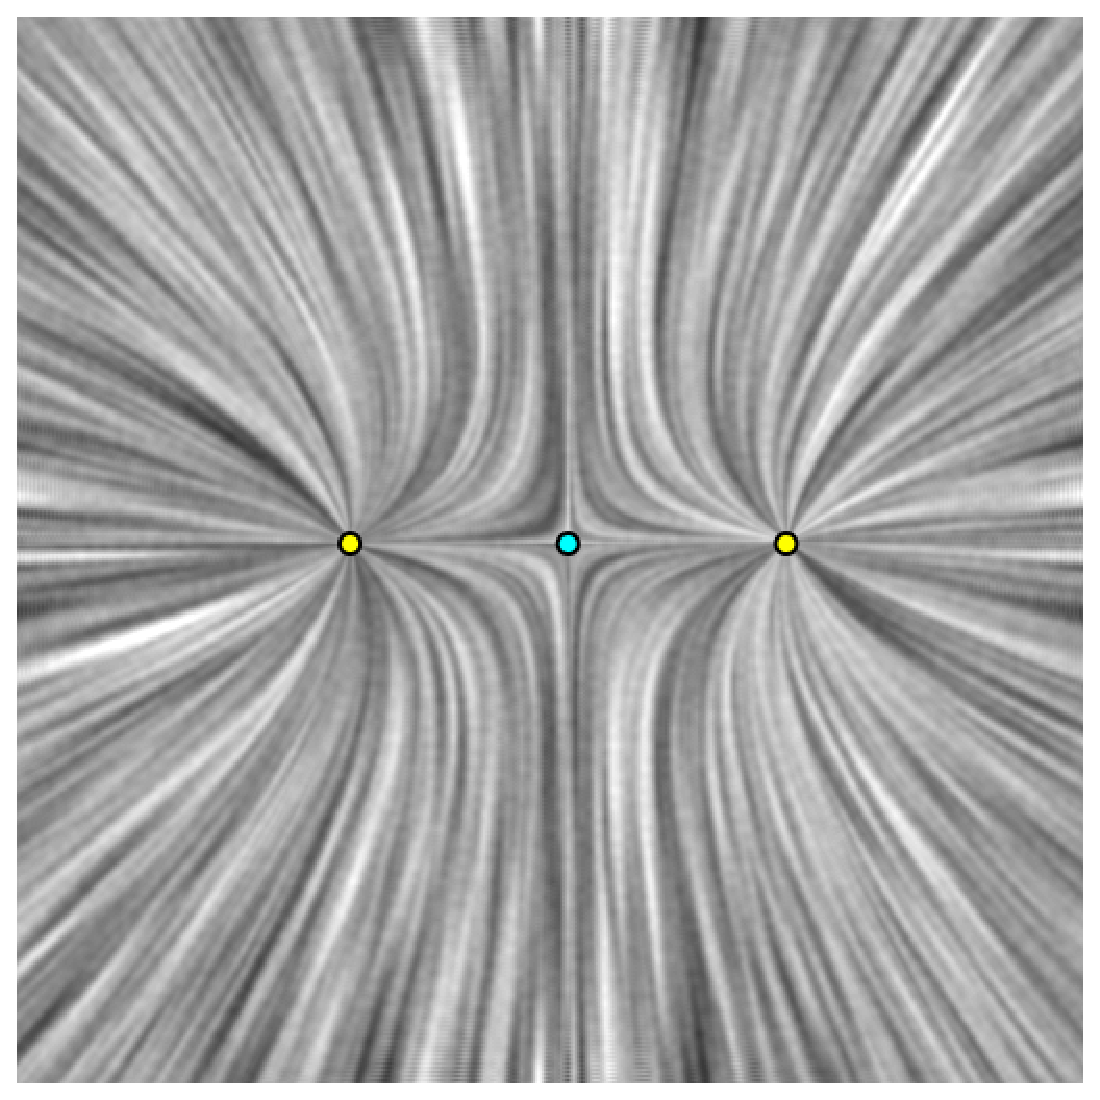
\includegraphics[height=1.07in]{images/cancel_step0_1sym.eps}
    \\
    \end{array}$
\end{center}
\caption{ A comparison between a $4$-RoSy field (left) and its
representation vector field (right). Notice that the sets of points
with a zero value are the same for both fields (colored dots).
Representation vectors remove the directional ambiguity in an
$N$-RoSy field. } \label{fig:vector_representation}
\end{figure}

\section{Topological Analysis of $N$-RoSy Fields}
\label{sec:analysis}

In this section, we describe important topological properties of
$N$-RoSy fields on manifold surfaces, such as {\em singularities}
and {\em separatrices}. We will also present efficient algorithms to
compute these quantities on mesh surfaces.

Singularity identification is necessary for providing explicit
control over the number and location of singularities, which is
needed in pen-and-ink sketching of 3D surfaces as undesirable
singularities cause visual artifacts~\cite{Hertzmann:00}
(Figures~\ref{fig:teaser} and~\ref{fig:result_pen_ink}). Singularity
and separatrix extraction allow better meshing near singularities
during the remeshing process (Section~\ref{sec:remeshing}).
Figure~\ref{fig:symmetry_separatrix_importance} illustrates this
with a 3D surface obtained by joining two cubes with rounded
corners. In the left, the singularities are highlighted by colored
dots and the separatrices are the colored curves emanating from the
singularities. Notice that singularities appear in natural places
(corners and joints) and separatrices indicate important directions
near the singularities. Utilizing separatrices during the remeshing
process produces meshes that can better maintain features in the
original mesh (Figure~\ref{fig:symmetry_separatrix_importance},
right) than disregarding them
(Figure~\ref{fig:symmetry_separatrix_importance}, middle).

The concepts of singularities and separatrices are well defined for
vector and tensor fields, i.e., when $N=1,2$. Next, we will extend
them to $N$-Rosy fields when $N \ge 3$.

\subsection{Singularities}
\label{sec:singularities}

For simplicity, consider a planar vector field $V(x, y) =
\begin{pmatrix} F(x, y) \\ G(x, y) \end{pmatrix}$. A {\em
singularity} ${\bf p}_0$ is a point in the domain where $V({\bf
p}_0)=0$. ${\bf p}_0$ is {\em isolated} if there exists an open
neighborhood $U$ of ${\bf p}_0$ with the property that ${\bf p}_0$
is the unique singularity in the interior of $U$ and there are no
singularities on the boundary of $U$. An isolated singularity ${\bf
p}_0$ can be characterized by its {\em Jacobian} $DV({\bf p}_0) =
\begin{pmatrix} a & b \\ c & d \end{pmatrix}$, where $a=\frac{\partial F}{\partial x}({\bf p}_0)$,
$b=\frac{\partial F}{\partial y}({\bf p}_0)$, $c=\frac{\partial
G}{\partial x}({\bf p}_0)$, and $d=\frac{\partial G}{\partial
y}({\bf p}_0)$. The {\em local linearization} of $V$ at a point
${\bf p}_0$ is a function $LV({\bf p}) = DV({\bf p}_0)({\bf p}-{\bf
p}_0)$.

%$\begin{pmatrix} r\cos\theta & r\sin\theta
%\end{pmatrix}^{\bf T}=DV({\bf p}_0)\begin{pmatrix} r\cos\theta &
%r\sin\theta
%\end{pmatrix}^{\bf T}$ where $(r, \theta)$ are the polar coordinates of
%displacement vectors in the neighhorhood of ${\bf p}_0$. Note that
%we intentionally used the polar coordinates in the definition of
%$LV$ .

We now consider how the angular component of a vector field changes
on an infinitesimal circle $\Gamma$ centered at ${\bf p}_0$. Given a
point ${\bf p} \in \Gamma$, we have ${\bf p} = {\bf p}_0 +
\begin{pmatrix} r\cos\theta \\ r\sin\theta \end{pmatrix}$
where $(r, \theta)$ are the polar coordinates. The local
linearization at ${\bf p}_0$ is
$LV({\bf p}) = r\begin{pmatrix} a\cos\theta+b\sin\theta \\
c\cos\theta+d\sin\theta
\end{pmatrix}$. The angular component is

\begin{equation}
\tan^{-1}(\frac{c\cos\theta+d\sin\theta}{a\cos\theta+b\sin\theta})
\end{equation}

\noindent which has a derivative


\begin{equation}
\frac{ad-bc}{(a\cos\theta+b\sin\theta)^2+(c\cos\theta+d\sin\theta)^2}
\end{equation}

\begin{figure}[t]
\begin{center}
    $\begin{array}{@{\hspace{-0.00in}}c@{\hspace{0.05in}}c@{\hspace{0.05in}}c}
%    \includegraphics[height=1.5in]{images/cubeU.eps}
    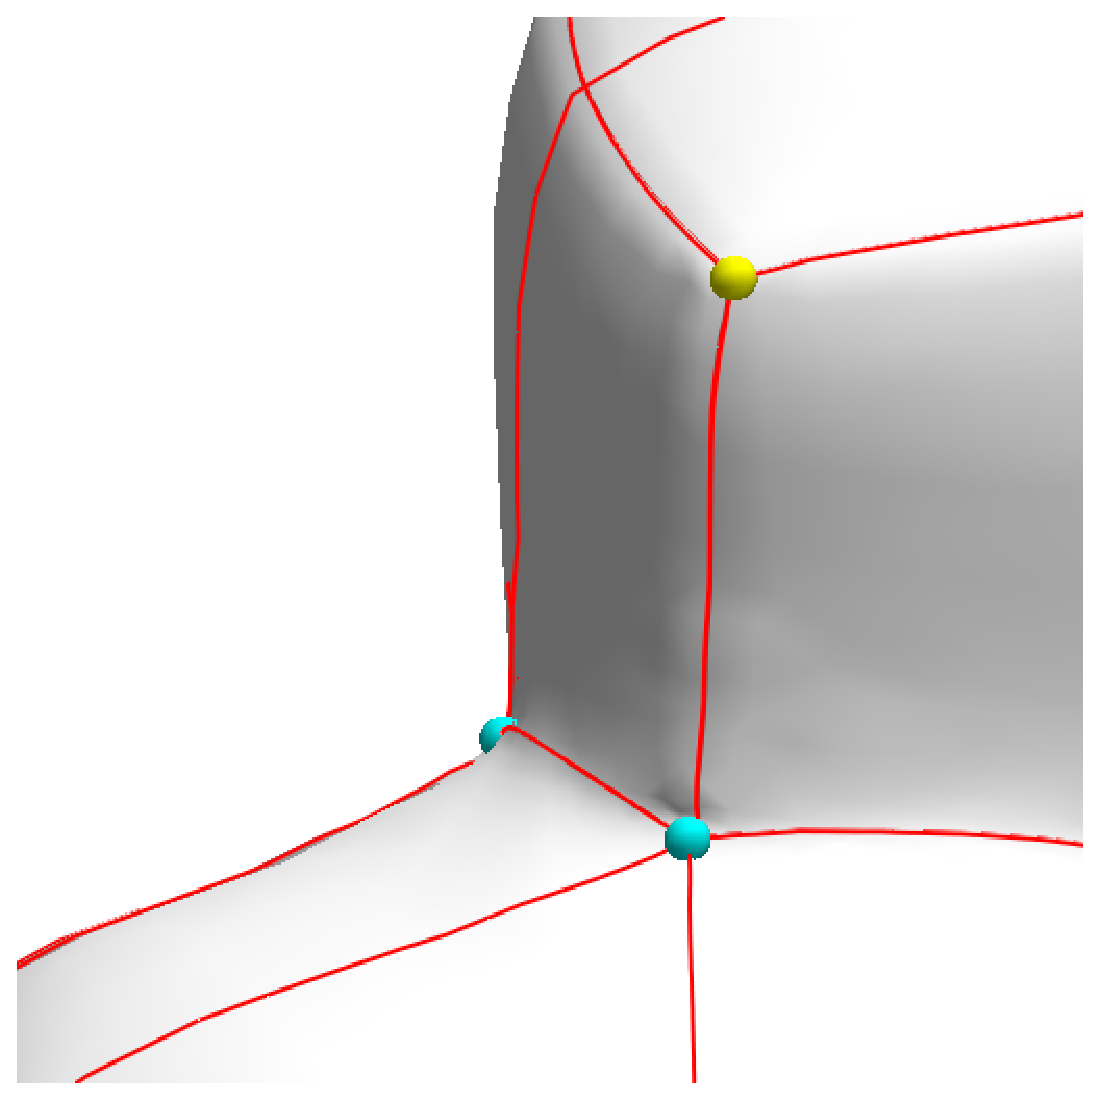
\includegraphics[height=1.1in]{images/cubeU_model_with_seps.eps}
    &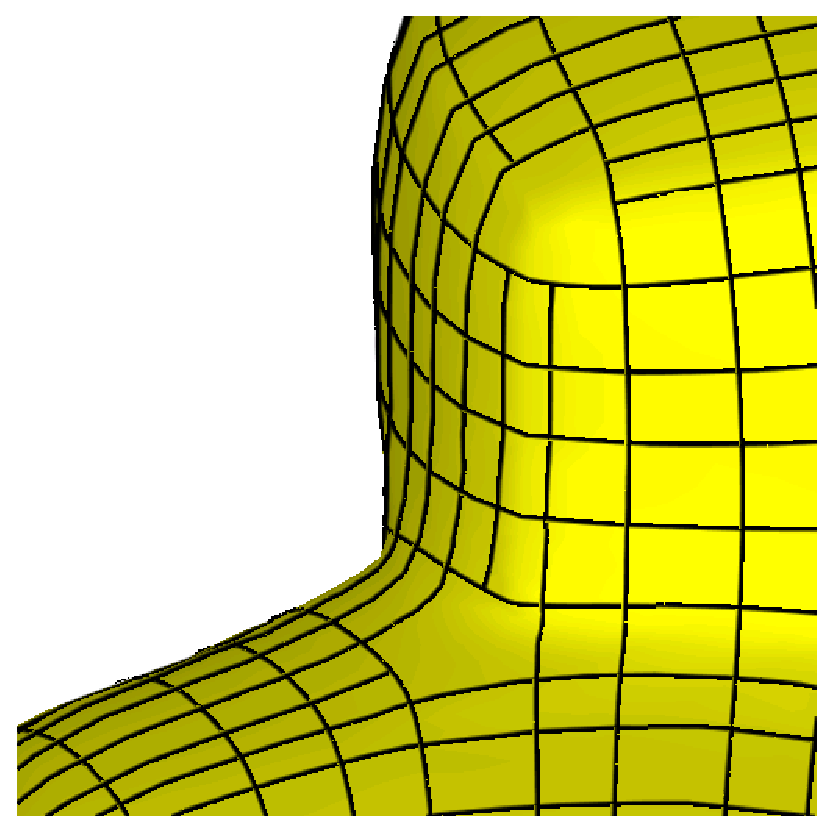
\includegraphics[height=1.1in]{images/cubeU_withoutSeps.eps}
    &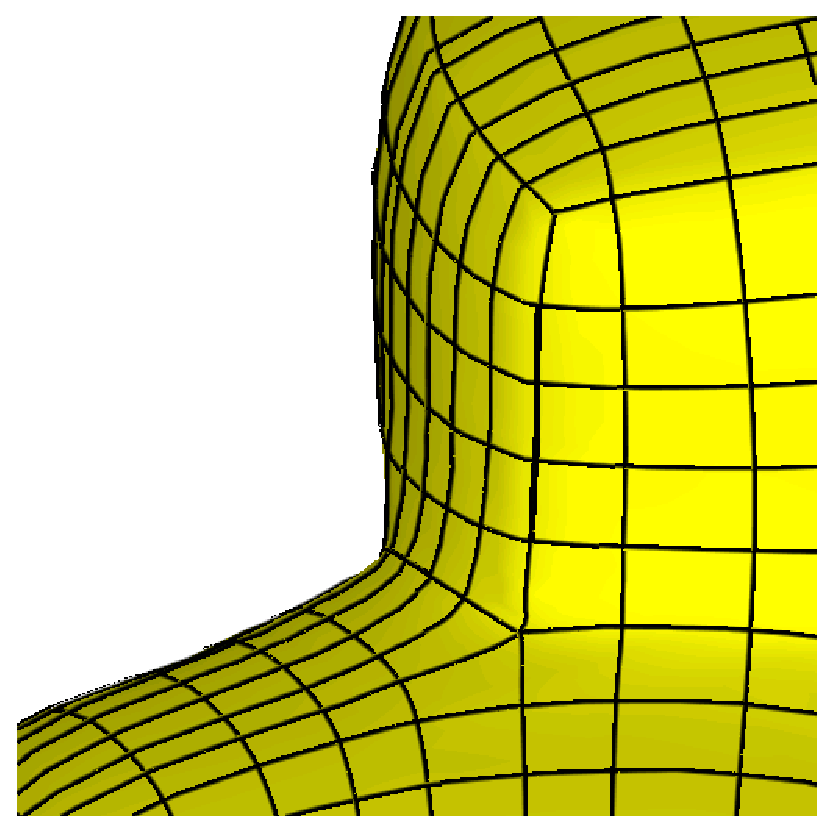
\includegraphics[height=1.1in]{images/cubeU_withSeps.eps}
    \\
    \end{array}$
\end{center}
\caption{ This figure illustrates the importance of singularity and
separatrix extraction in quad-dominant remeshing. Given a 3D model
(left), the singularities and separatrices are highlighted by
colored dots and curves, respectively. Including separatrices during
remeshing can lead to better meshes near the singularities (right)
than not including them (middle). }
\label{fig:symmetry_separatrix_importance}
\end{figure}

%Therefore, the angular component is monotonically increasing
%(decreasing) if $ad-bc > 0$ ($ad-bc < 0$). In fact,
When $ad-bc \ne 0$, the sign of the quantity $ad-bc$ is related to
the {\em Poincar\'e index} of ${\bf p}_0$, which is defined in terms
of the {\em winding number} for the {\em Gauss map}.

Let $V$ be a continuous planar vector field and $D_0 \subset
\mathbb{R}^2$ be the zero set for $V$. The {\em Gauss map}
$\epsilon: \mathbb{R}^2 \setminus{D_0} \to S^1$ is defined as
$\epsilon(x) = \frac{V(x)}{\arrowvert V(x) \arrowvert}$. $\epsilon$
is continuous in $\mathbb{R}^2 \setminus{D_0}$. In particular, it
introduces a continuous map $\epsilon|_{\Gamma}$ on any simple loop
$\Gamma$ that does not contain any singularity. When traveling along
$\Gamma$ in the positive direction once, the image under
$\epsilon|_{\Gamma}$ necessarily covers the unit circle $S^1$ an
integer number of times counting orientation. This integer is the
{\em winding number} of $V$ along $\Gamma$. The Poincar\'e index of
an isolated singularity ${\bf p}_0$ is the winding number of any
simple loop that encloses ${\bf p}_0$ and contains no other
singularities either in its interior or on the boundary. Denote this
number as $\kappa(V;{\bf p}_0)$. The Poincar\'e index is $+1$ for
sources, sinks, centers, and foci. It is $-1$ for saddles, and $0$
for regular points.

The {\em Poincar\'{e}-Hopf theorem} links the topology of a vector
field to that of the underlying domain in the following way. Let $M$
be a closed orientable manifold with an Euler characteristic
$\chi(M)$. Furthermore, let $V$ be a continuous vector field defined
on $M$ with only isolated singularities ${\bf p}_1,..., {\bf p}_n$.
Then

\begin{equation}
\sum_{i=1}^{n}\kappa(V;{\bf p}_i)=\chi(M)
\end{equation}.
%An immediate corollary
%of the Poincar\'{e}-Hopf theorem is that given a particular vector
%field $V$, if one wants to remove a singularity of a positive or
%negative Poincar\'e index, then one must simultaneously remove a
%singularity of the opposite sign. In fact, for a 2-manifold, a zero
%total Poincar\'e index for a region $R$ guarantees that it is
%possible to replace the vector field inside $R$ with a
%singularity-free vector field.
%
%A positive-indexed singularity can be a source, a sink, a center, or
%a focus. A negative-indexed singularity is a saddle.

We now extend the concepts of singularities to $N$-RoSy fields where
$N \ge 2$. Given a planar $N$-RoSy field $S$, we define $V_S({\bf
p}) = \gamma (S({\bf p}))$ as the {\em representation vector field}
of $S$. Then, a point ${\bf p}_0$ is an isolated singularity of $S$
if and only if it is also an isolated singularity of $V_S$. We
define the index of a singularity ${\bf p}_0$ with respect to $S$ as

\begin{equation}
\kappa(S; {\bf p}_0) = \frac{\kappa(V_S; {\bf p}_0)}{N}
\end{equation}

A singularity ${\bf p}_0$ is of {\em $L$-th order} if its index is
$|\frac{L}{N}|$. ${\bf p}_0$ is {\em positive}, {\em negative}, or
{\em regular} if $\kappa(S; {\bf p}_0) > 0$, $\kappa(S; {\bf p}_0) <
0$, or $\kappa(S; {\bf p}_0) =0$, respectively. As in the case of
vector fields and tensor fields, an $L$-th order singularity can be
constructed by clustering $L$ first-order
singularities~\cite{Scheuermann:98,Delmarcelle:94}. Assuming an
$N$-RoSy field has first-order singularities only, $N|\chi(M)|$
provides a lower bound on the number of singularities in the field.
While more singularities can occur, their signed sum remains
constant, i.e., $\chi(M)$.

Figure~\ref{fig:symmetry_examples} shows natural symmetries on the
Platonic solids. To understand what symmetry is natural in a shape,
let us consider the total angle around a vertex of the cube, which
is $\frac{3\pi}{2}$. In order to admit continuity across such a
corner, one must accept a rotation of $\frac{\pi}{2}$, which is
essentially the case when $N=4$. Similarly, an octahedron naturally
admits $3$-RoSy's, an icosahedron admits $6$-RoSy's, a dodecahedron
admits $10$-RoSy's, and a tetrahedron admits $2$-RoSy's (tensors).
In all these cases, there are $K$ first-order positive singularities
where $K$ is the number of vertices in the shape. Furthermore, the
total signed index sum is $2$, which is the Euler characteristic of
a genus-zero surface. Let $\beta$ be the {\em angle of deficit} of a
vertex, which equals $2\pi$ minus the total angle around the vertex.
$\beta \ne 0$ implies that the neighborhood of the vertex is likely
to admit an $N=\frac{2\pi}{|\beta|}$ symmetry. When $\beta > 0$, the
vertex is a positive singularity, and when $\beta < 0$, the vertex
is a negative singularity. Next, we discuss the separatrices in an
$N$-RoSy field.

\subsection{Separatrices}
\label{sec:separatrices}

A {\em separatrix} in a vector field is a trajectory that passes
through a saddle. The {\em topology} of a vector field on a
two-dimensional surface consists of singularities and separatrices.
Extending the definition of {\em separatrices} to $N$-RoSy fields
when $N \ge 2$ is more difficult because separatrices can emanate
from singularities with a positive index. To address this,
Delmarcelle and Hesselink~\shortcite{Delmarcelle:94} define
separatrices for a tensor field ($2$-RoSy) as the boundaries of a
{\em hyperbolic sector}, which is a region in the vicinity of a
singularity inside which trajectories sweep pass the singularity. As
an example, there are four hyperbolic sectors for every saddle.

We adopt this approach and define separatrices of an $N$-RoSy field
$S$ as the boundary of a hyperbolic sector for a singularity.
Figure~\ref{fig:symmetry_separatrix_definition} (a-d) show the four
hyperbolic sectors for a positively-indexed singularity in a
$3$-RoSy field, and (e) their composition. The red lines are {\em
incoming separatrices} and the green lines are {\em outgoing
separatrices}. In (f) we show the separatrices of a negatively-index
singularity in a $4$-RoSy field. When $N$ is even, separatrices do
not have directions. Notice when $N \ge 3$, hyperbolic sectors can
overlap, which is a reflection of the fact that there are $N$ member
vectors. When $N$ is even, there are $\frac{N}{2}$ streamlines
passing through every non-singular point. When $N$ is odd, there are
$N$ such streamlines.

To extract separatrices, we make use of the following observation: a
separatrix approaches a singularity in a radial direction. In other
words, given an isolated singularity ${\bf p}_0$, we consider its
local linearization $DS = \begin{pmatrix} a & b \\ c & d
\end{pmatrix}$, which is defined in terms of the linearization of
the representation vector field. On an infinitesimal circle centered
at ${\bf p}_0$, we consider directions $v = {\bf p} - {\bf p}_0$
such that $v$ is also a member vector at ${\bf p}$. Let $\phi$ be
the angular coordinate of one of the member vectors. The
aforementioned statement is equivalent to finding directions $v =
\begin{pmatrix} \cos\theta \\ \sin\theta \end{pmatrix}$ such
that

\begin{equation}
N\theta \equiv N\phi \mod 2\pi
\end{equation}

\noindent which can be used to find a separatrix that passes through
the singularity. Note that this is consistent with the definitions
of separatrices in vector fields~\cite{Tricoche:02} and tensor
fields~\cite{Delmarcelle:94}. The condition can be rewritten as

\begin{equation}
\frac{\sin N\theta}{\cos N\theta} =
\frac{c\cos\theta+d\sin\theta}{a\cos\theta+b\sin\theta}
\label{eq:sep_computation}
\end{equation}

Recall that

\begin{eqnarray}
\cos N\theta =
\sum_{i=0}^N{\cos\frac{i\pi}{2}
\begin{pmatrix} N \\ i \end{pmatrix} \cos^{N-i}\theta\sin^i\theta} \\ \sin N\theta =
\sum_{i=0}^N{\sin\frac{i\pi}{2} \begin{pmatrix} N \\ i
\end{pmatrix} \cos^{N-i}\theta\sin^i\theta}
\end{eqnarray}.

\noindent Consequently, solving Equation~\ref{eq:sep_computation}
amounts to finding the roots of an $(N+1)$-th order polynomial.
%
%\noindent or
%
%\vspace{-0.2in}
%
%\begin{equation}
%\sin N\theta (a\cos\theta+b\sin\theta) = \cos N\theta
%(c\cos\theta+d\sin\theta) \label{eq:sep_computation}
%\end{equation}
%
%\vspace{-0.2in}


%\vspace{-0.2in}
%
%\begin{equation}
%\alpha_i = \left\{ \begin{array}{ll} \quad 1 & \textrm{ if $i \equiv 0 \mod 4$} \\
%-1 & \textrm{ if $i \equiv 2 \mod 4$} \\
%\quad 0 & \textrm{ otherwise}
%\end{array} \right.
%\end{equation}
%
%\vspace{-0.2in}
%
%\noindent and
%
%\vspace{-0.2in}
%
%\begin{equation}
%\beta_i = \left\{ \begin{array}{ll} \quad 1 & \textrm{ if $i \equiv
%1 \mod 4$}
%\\ -1 & \textrm{ if $i \equiv 3 \mod
%4$ } \\ \quad 0   & \textrm{ otherwise}
%\end{array} \right.
%\end{equation}
%
%\vspace{-0.2in}
A first-order negative singularity has $N+1$ separatrices while a
first-order positive singularity has at most $N+1$ separatrices.
Note that the above definition extracts all the separatrices in an
$N$-RoSy field $S$ only when $N$ is even. In case $N$ is odd, the
solutions to Equation~\ref{eq:sep_computation} correspond to the
outgoing separatrices only. To capture the incoming separatrices, we
need to compute the solutions to

\begin{equation}
N\theta \equiv N\phi+\pi \mod 2\pi
\end{equation}

\noindent which is equivalent to computing the separatrices of $-S$.
Next, we describe how we represent an $N$-RoSy field on a triangular
mesh surface and how to extract the topological features in the
discrete setting.

\begin{figure}[t]
\begin{center}
    $\begin{array}{@{\hspace{-0.00in}}c@{\hspace{0.05in}}c@{\hspace{0.05in}}c@{\hspace{0.05in}}c}
    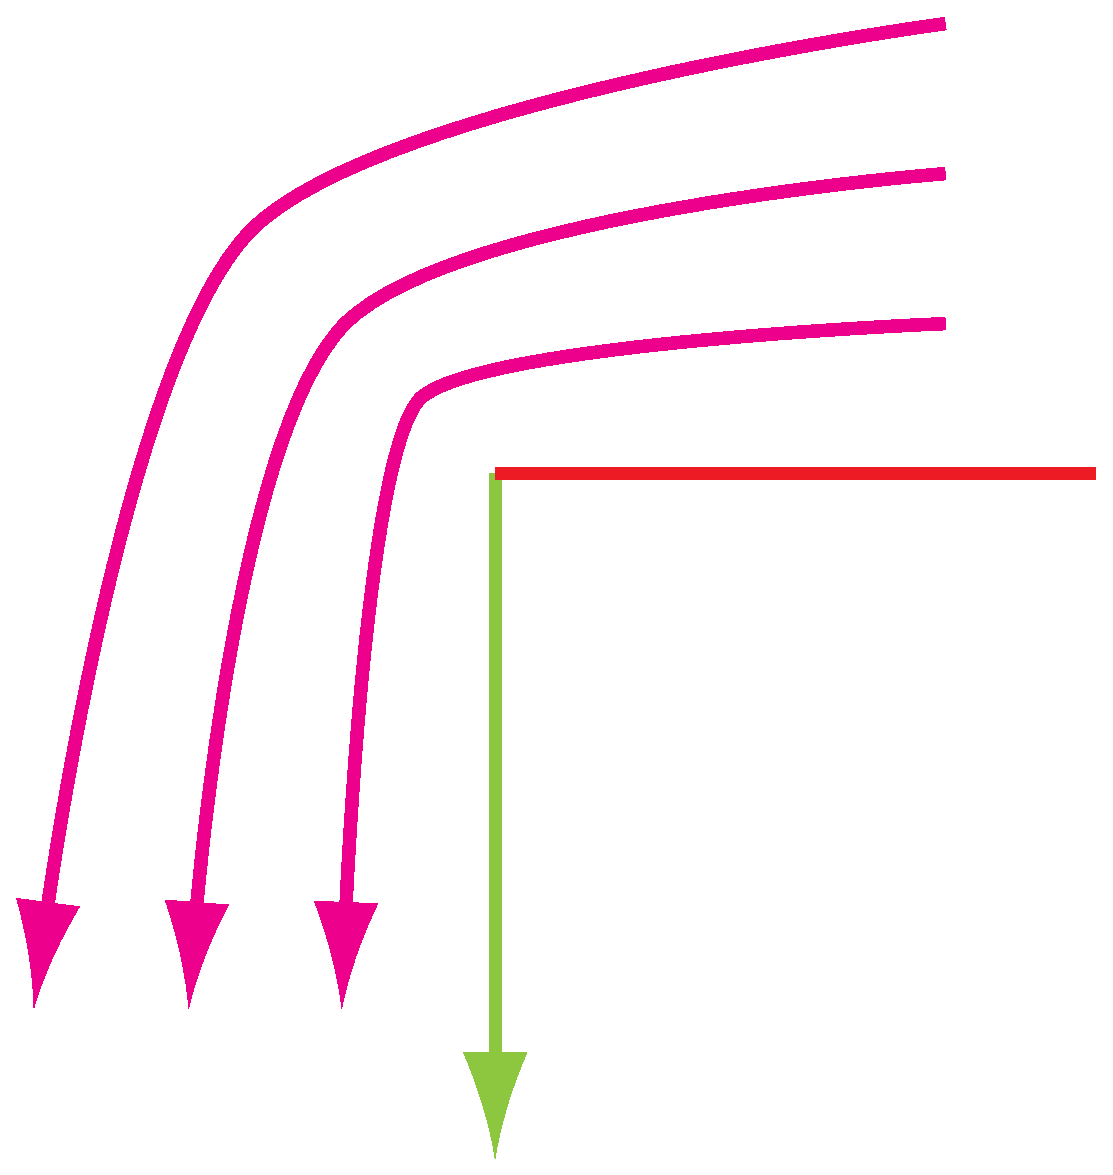
\includegraphics[height=1.1in]{images/3_separatrices_0.eps}
    &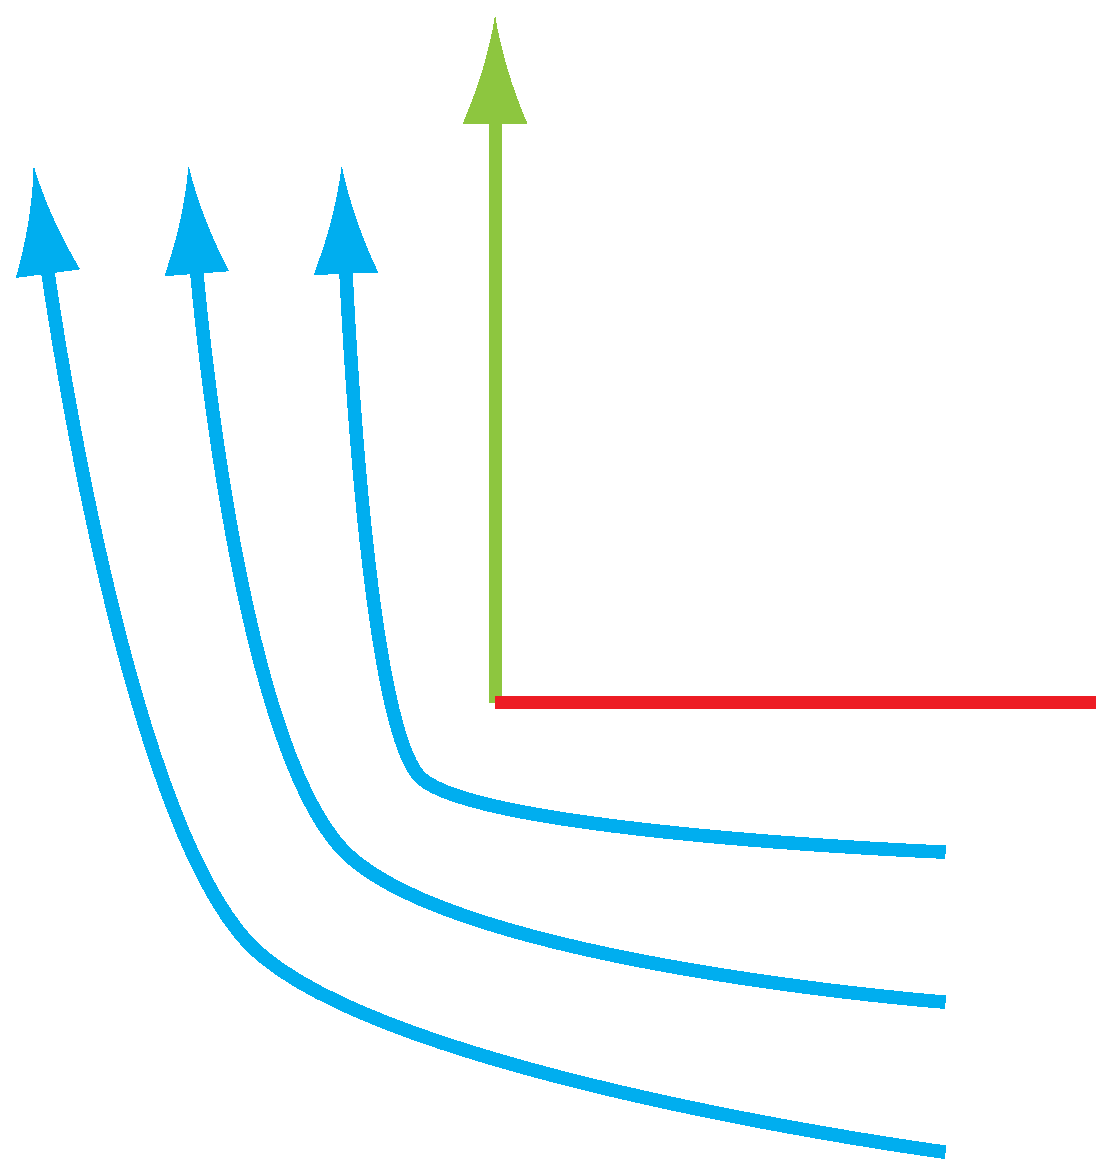
\includegraphics[height=1.1in]{images/3_separatrices_1.eps}
    &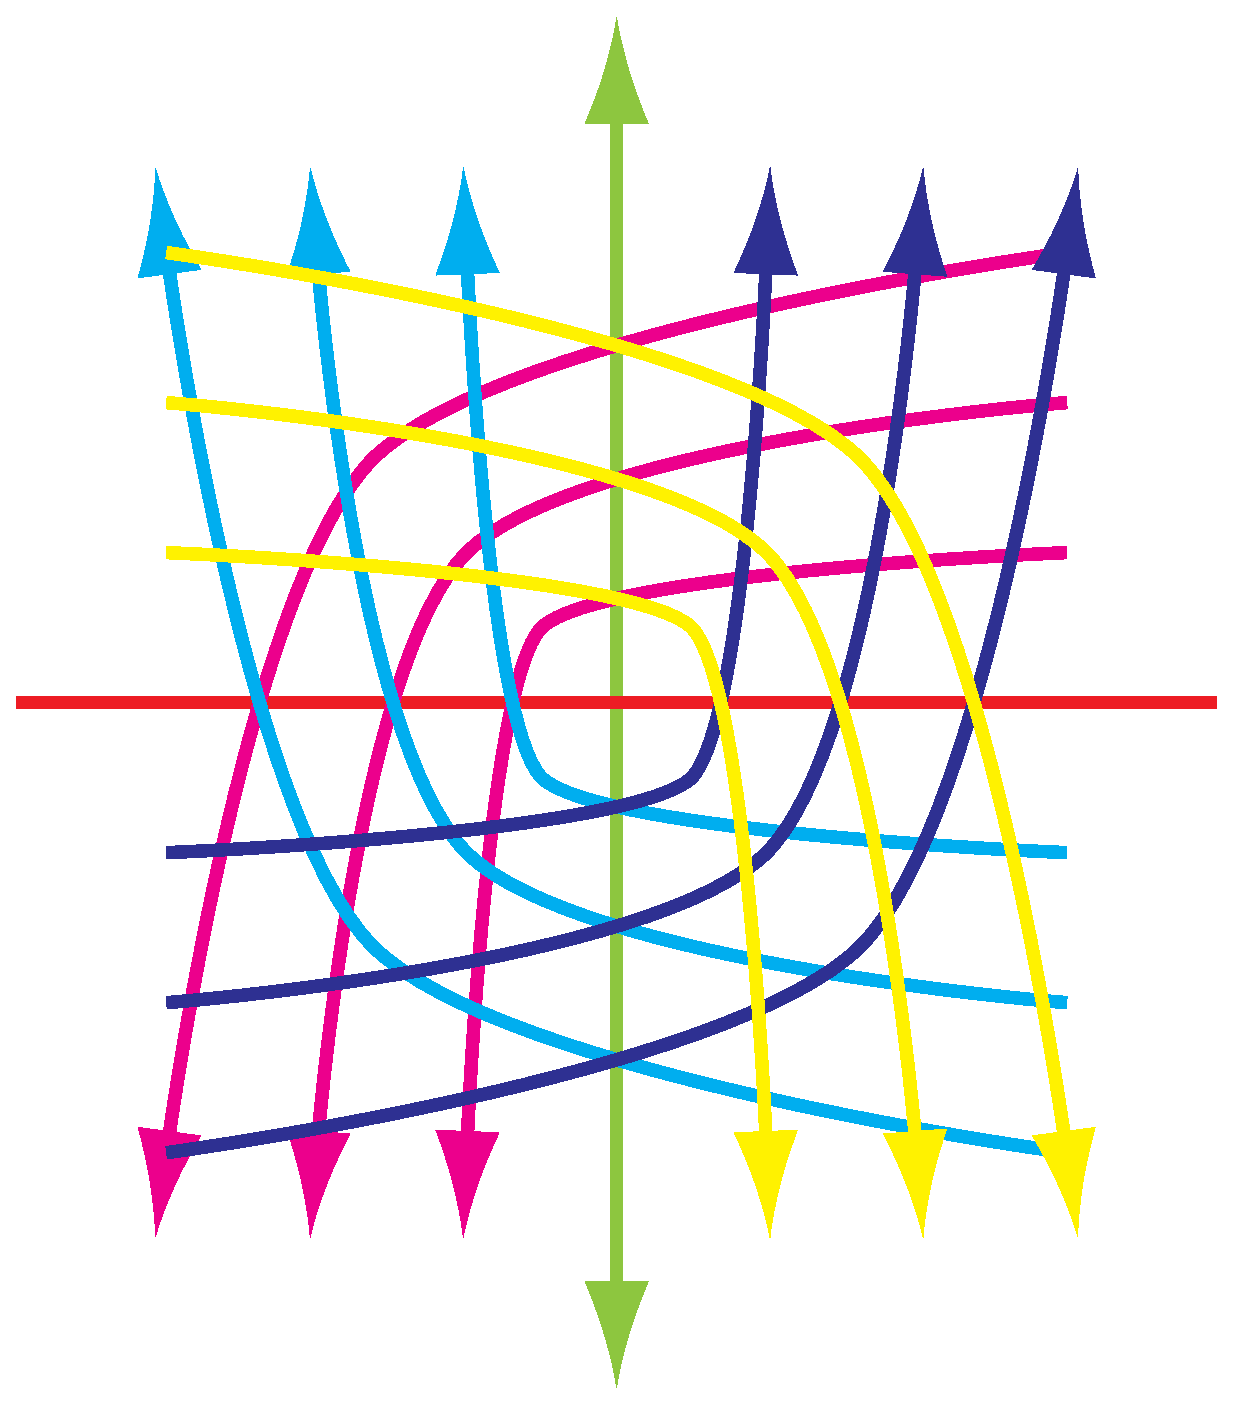
\includegraphics[height=1.1in]{images/3_separatrices.eps}
    \\
    (a) & (b) & (e) \\
    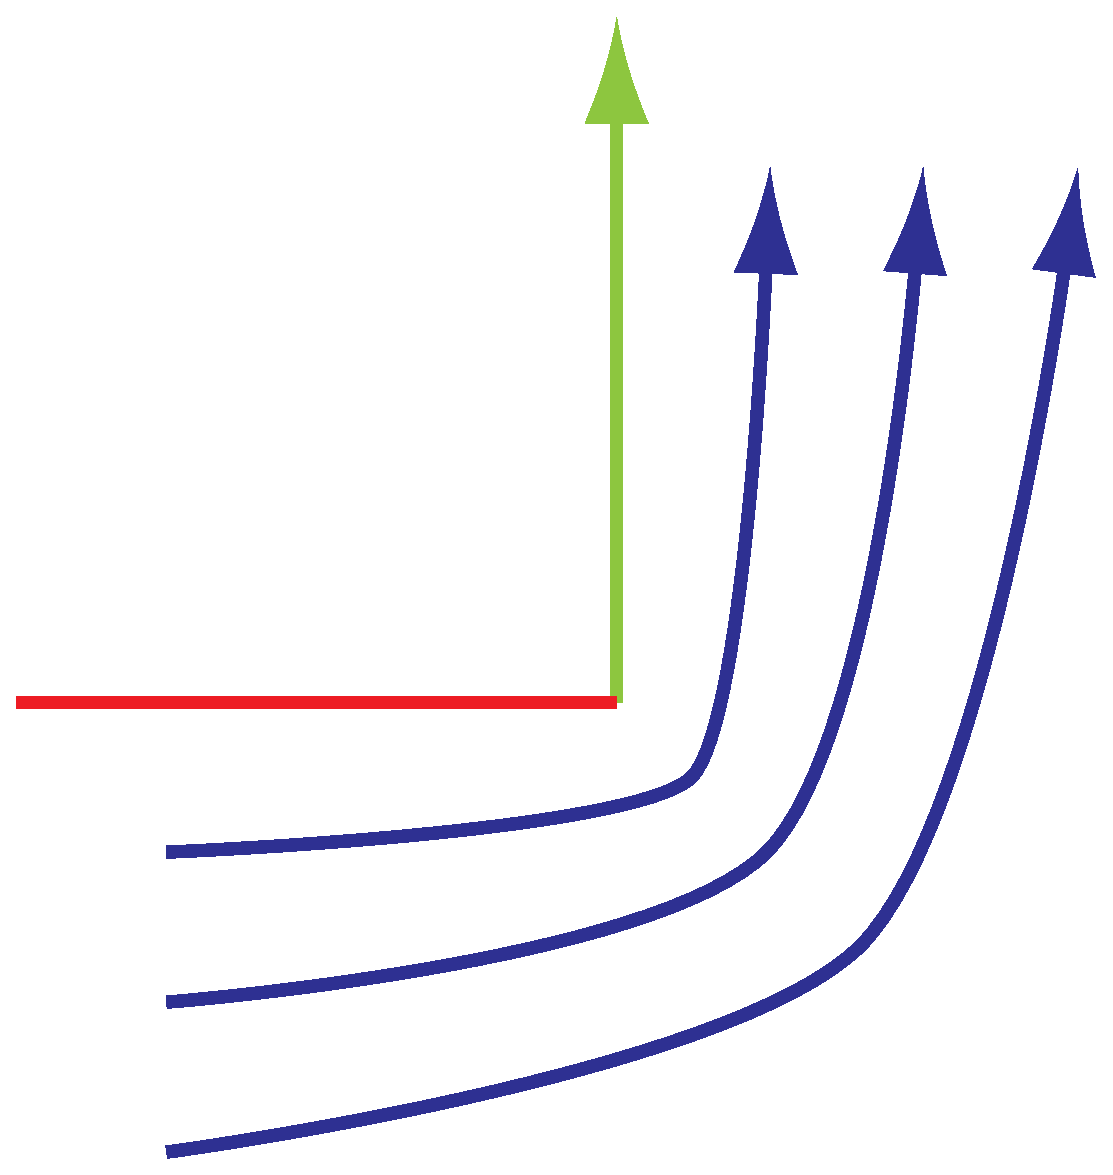
\includegraphics[height=1.1in]{images/3_separatrices_2.eps}
    &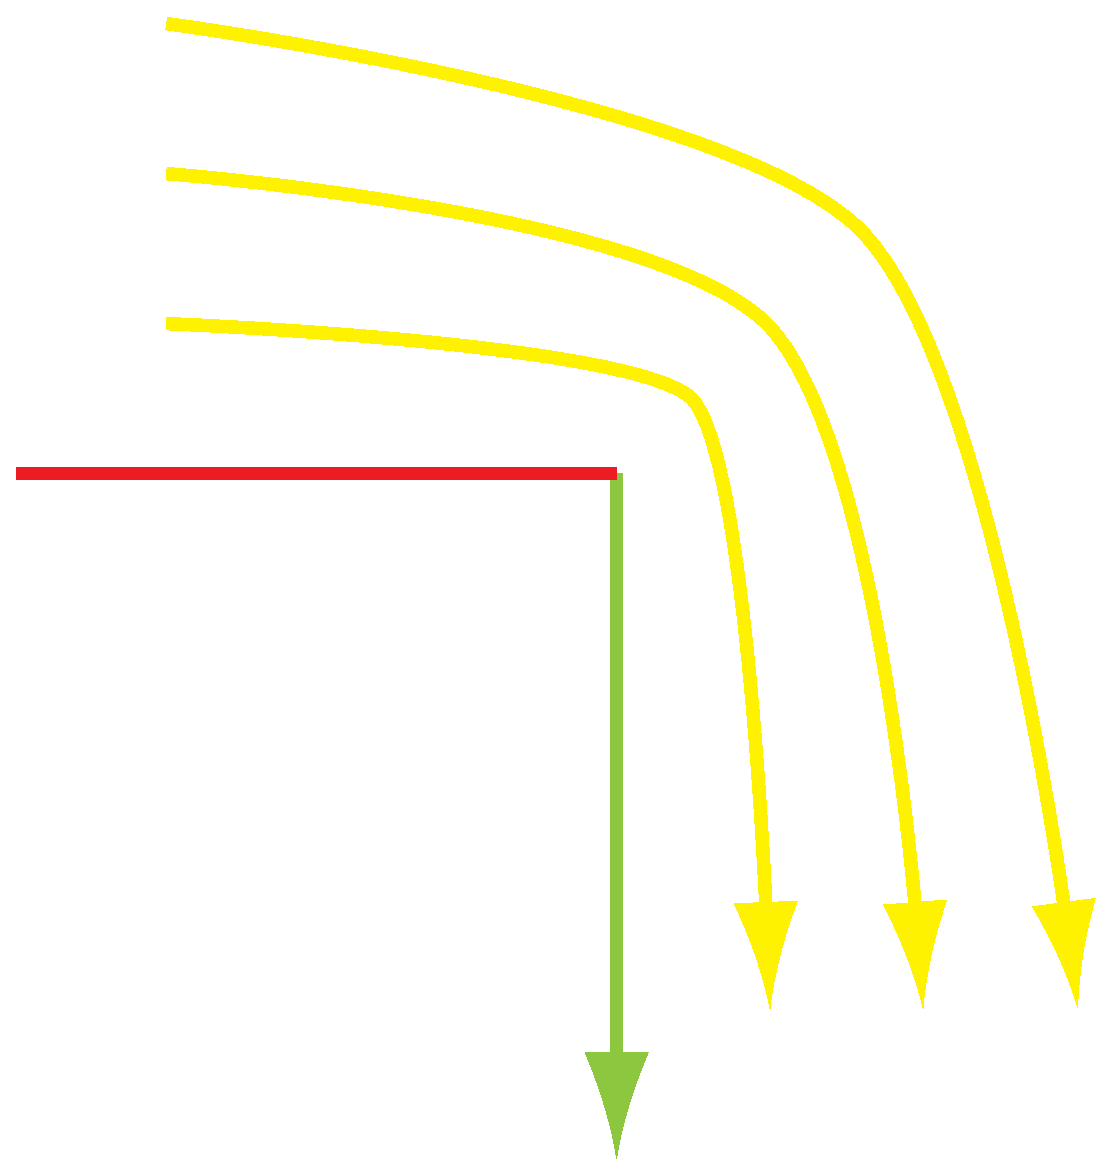
\includegraphics[height=1.1in]{images/3_separatrices_3.eps}
    &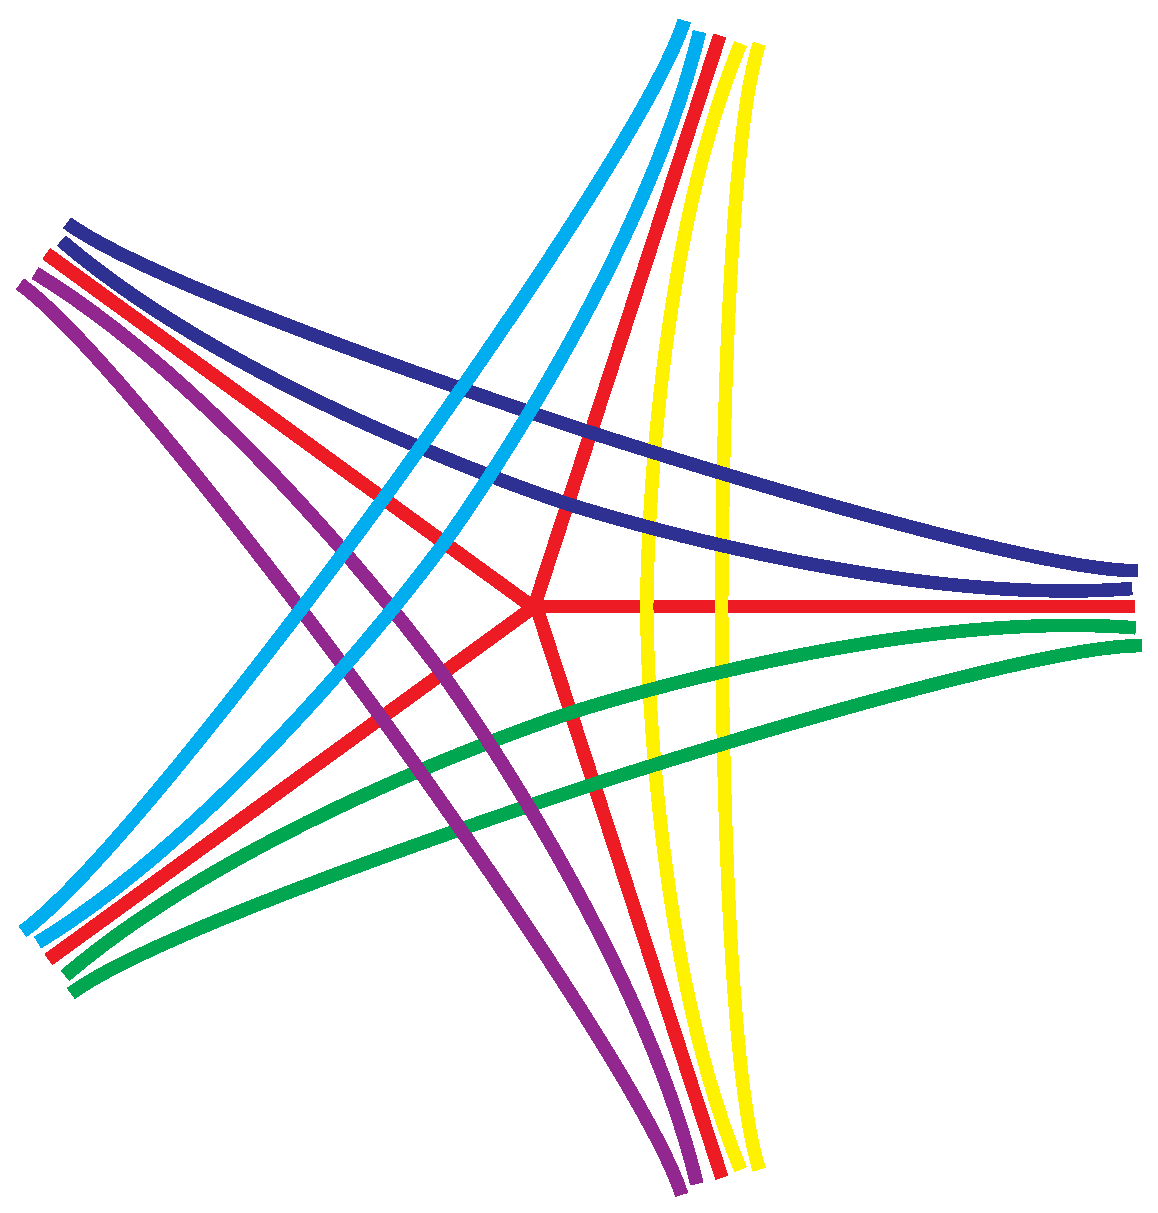
\includegraphics[height=1.1in]{images/4_separatrices.eps}
    \\
    (c) & (d) & (f) \\
    \end{array}$
\end{center}
\caption{ The separatrices of an $N$-RoSy field are the boundaries
of the hyperbolic sectors in the vicinity of a singularity. In
(a)-(d), we show the four hyperbolic sectors for a positive
singularity of a $3$-RoSy field. These sectors overlap and each of
them has an incoming separatrix (red line) and an outgoing
separatrix (green line). Together, they describe the topology of the
field near the singularity (e). In (f), we show the separatrices for
a negative singularity in a $4$-RoSy field. Notice that separatrices
do not have directions when $N$ is even.  }
\label{fig:symmetry_separatrix_definition}
\end{figure}

\subsection{Discrete Representation}
\label{sec:represent}

On a triangular mesh, we use a vertex-based representation for an
$N$-RoSy field $S$. In such a setting, the values of $S$ are defined
at the vertices and interpolations are used to obtain values on
edges and inside triangles. Note that in practice we use the
representation vector field $V_S$ instead of $S$ itself.

When the triangular mesh represents a planar domain, we use the
popular piecewise linear interpolation scheme of vector
fields~\cite{Tricoche:02}. Basically, inside every triangle the
representation vector field $V_S$ is {\em linear} and therefore can
be expressed as $\begin{pmatrix} ax+by+e \\ cx+dy+f
\end{pmatrix}$ under the global coordinate systems. Here,
$\begin{pmatrix} a & b \\ c & d \end{pmatrix}$ is the Jacobian of
the representation vector field, and it is constant inside every
triangle. This representation supports efficient singularity and
separatrix extraction. We perform the following steps in computing
the topology of an $N$-RoSy field.

\begin{enumerate}
%\itemsep 0pt
%\parskip -1pt
\item We locate the singularities of the representation vector
field using the method in~\cite{Tricoche:02} and compute the
linearization, which is constant for each triangle.
\item We extract separatrix directions by solving
Equation~\ref{eq:sep_computation} for every singularity.
\item For each separatrix direction $w$, we perform
streamline tracing from a point sufficiently close to the
singularity in the direction of $w$.
\end{enumerate}

On meshes that represent curved surfaces, the above piecewise linear
scheme no longer produces continuous $N$-RoSy fields. We refer the
readers to~\cite{Zhang:06} for an example when $N=1$. Furthermore, a
curved surface in general lacks a global parameterization and
consistent local frames. To overcome these problems, Zhang et
al.~\shortcite{Zhang:06} develop a non-linear interpolation scheme
that produces continuous vectors fields and supports efficient
singularity and separatrix extraction. Their scheme is based on the
ideas of {\em geodesic polar maps} and {\em parallel transport} from
differential geometry. Extending this scheme to $N$-RoSy fields is
straightforward, and it has been done when $N=2$~\cite{Zhang:07}.
Recently, Wang et al.~\shortcite{Wang:06} have proposed another
scheme based on edge subdivision and discrete differential forms.
Adapting their scheme to $N$-RoSy fields is also promising.

%\begin{figure*}[t]
%\begin{center}
%    $\begin{array}{@{\hspace{-0.00in}}c@{\hspace{0.02in}}c@{\hspace{0.02in}}c@{\hspace{0.1in}}c@{\hspace{0.1in}}c}
%    \includegraphics[width=1.35in]{images/3_0_a.eps}
%    &\includegraphics[width=1.35in]{images/3_1_a.eps}
%    &\includegraphics[width=1.35in]{images/3_2_a.eps}
%    &\includegraphics[width=1.35in]{images/3_a.eps}
%    &\includegraphics[width=1.35in]{images/weightImg.eps}\\
%    (1a) \quad \phi = 0  &   (2a) \quad \phi = \frac{2\pi}3  &  (3a) \quad \phi = \frac{4\pi}3 &  (c) \quad (1a+2a+3a)/3 & (e) \quad weight \\
%    \\
%    \includegraphics[width=1.35in]{images/3_0_b.eps}
%    &\includegraphics[width=1.35in]{images/3_1_b.eps}
%    &\includegraphics[width=1.35in]{images/3_2_b.eps}
%    &\includegraphics[width=1.35in]{images/3_b.eps}
%    &\includegraphics[width=1.35in]{images/3_final.eps}\\
%    (1b) \quad \phi = \frac{\pi}6  &   (2b) \quad \phi = \frac{3\pi}6 &  (3b) \quad \phi = \frac{5\pi}6 &  (d) \quad (1b+2b+3b)/3  & (f) \quad c \times e+d \times (1-e) \\
%\end{array}$
%\end{center}
%\caption{ Our visualization algorithm is demonstrated with an
%example $3$-RoSy field $S$. From (1a)-(3a), we applied the IBFV
%algorithm to $V_{S, 0}$, $V_{S, \frac{2\pi}{3}}$, and $V_{S,
%\frac{4\pi}{3}}$, respectively. The green line segments shown in
%these images indicate $\phi$ and the black line segments show the
%ranges that are used to select member vectors. Notice that while
%(1a)-(3a) provide a complete coverage of the streamlines passing
%through any regular point in the domain, they have the same regions
%of breaking points (left $X$-axis). By blending them uniformly, we
%obtained a visualization of $S$ with visual artifacts in the same
%place. To remedy the problem, we also applied the IBFV algorithm to
%$V_{S, \frac{\pi}{6}}$ (1b), $V_{S, \frac{3\pi}{6}}$ (2b), and
%$V_{S, \frac{5\pi}{6}}$ (3b), and blended them uniformly to obtain
%(d). The visual artifacts in (d) appear on the right side of the
%$X$-axis. By blending them using the weight map (e), we obtain the
%final image in (f) that is artifact-free. \vspace{-0.1in} }
%\label{fig:symmetry_vis}
%\end{figure*}

%\section{Visualization of $N$-RoSy Fields}
%\label{sec:visualization}
%
%\vspace{-0.2in}
%
%In this section, we describe our visualization method for $N$-RoSy
%fields on the plane and surfaces. It is adapted from the Image-Based
%Flow Visualization (IBFV) technique~\cite{vanWijk:02} for vector
%fields, which we have chosen due to its impressive combination
%of speed and quality. To use IBFV, we need to define a vector field
%based on an $N$-RoSy field. This is done by choosing a member vector
%everywhere in the domain. However, there are two fundamental
%difficulties that need to be addressed.
%
%First, a member vector field is in general discontinuous as a vector
%field when $N \ge 2$. To see this, consider a first-order positive
%singularity, whose tensor index is $\frac{1}{N}$. When traveling
%around a small circle surrounding the singularity, the vector values
%on the small circle will cover $\frac{2\pi}{N}$ instead of $2\pi$.
%This leads to jumps in the vector values
%(Figure~\ref{fig:symmetry_vis}, 1a). Note that the discontinuity is
%not present in the $N$-RoSy field but a mere product of the
%topological differences between a vector field and an $N$-RoSy
%field.
%
%Second, there is more than one streamline passing through a
%regular point when $N \ge 3$, which suggests that visualizing a
%member vector field can be incomplete and incoherent. In
%Figure~\ref{fig:symmetry_vis}, six ways of converting an $3$-RoSy
%field into a vector field are shown (1a-3a, 1b-3b). Notice that it
%is difficult to judge whether two such plots correspond to the same
%$N$-RoSy field, let alone identify the features in the field.
%
%To address these issues, we convert an $N$-RoSy field in a number of
%different vector fields and blend the resulting IBFV-style images.
%By using a carefully designed scheme, we ensure that all the
%streamline directions for any regular point are present and that
%regions of artificial discontinuities are hidden. Before describing
%the details of our algorithm, we need the following definitions.
%
%Given an $N$-RoSy $s = \{R\begin{pmatrix} \cos(\theta +
%\frac{2k\pi}{N}) & \sin(\theta + \frac{2k\pi}{N}) \end{pmatrix}^{bf
%T} \mid 0 \le k \le N-1 \}$ and an angle $\phi \in [0, 2\pi)$, we
%define $l_{s, \phi} = \min_{k} |\theta+\frac{2k\pi}{N} - \phi|$ and
%$v_{s, \phi} = R\begin{pmatrix} \cos(\theta + \frac{2l_{s,
%\phi}\pi}{N}) & \sin(\theta + \frac{2l_{s, \phi}\pi}{N})
%\end{pmatrix}^{\bf T}$. $v_{s, \phi}$ is the member vector of $s$ that has
%the smallest angle with respect to the vector $v_0 = \begin{pmatrix}
%\cos\phi & \sin\phi \end{pmatrix}^{\bf T}$. When there are two
%minima, we choose the one such that $\theta+\frac{2k\pi}{N} - \phi >
%0$. In this case, we refer to $\phi$ as a {\em breaking angle} for
%$s$. It is straightforward to verify the following facts.
%
%\begin{enumerate}
%\itemsep 0pt
%\parskip -1pt
%\item $s = \{v_{s, \phi+\frac{2k\pi}{N}} \mid 0 \le k \le N-1 \}$
%for any $\phi$. \label{ob:rule1}
%\item $v_{s, \phi} = - v_{s, \phi+\pi}$. \label{ob:rule2}
%\item If $\phi$ is a breaking angle for $s$, so are $\phi + \frac{2k\pi}{N}$
%for any $k \in \mathbb{Z}$. \label{ob:rule3}
%\item If $\phi$ is a breaking angle for $s$, then $\phi + \frac{(2k+1)\pi}{N}$ is
%not a breaking angle for any $k \in \mathbb{Z}$. \label{ob:rule4}
%\end{enumerate}
%
%Given an $N$-RoSy field $S$, we define a vector field $V_{S,
%\phi}({\bf p}) = -v_{S({\bf p}), \phi}$. When $N$ is odd, we choose
%two sets of $L$ vector fields: $V_1 = \{ V_{S, \frac{2k\pi}{N}} \mid
%0 \le k \le N-1 \}$ and $V_2 = \{ V_{S, \frac{(2k+1)\pi}{N}} \mid 0
%\le k \le N-1 \}$. Note that both $V_1$ and $V_2$ form a complete
%coverage of all the streamline directions
%(Observation~\ref{ob:rule1}) and they have the same regions of
%visual discontinuity (Observation~\ref{ob:rule3}). Furthermore, the
%intersection of the sets of discontinuity according to a vector
%field from $V_1$ and a vector field from $V_2$ consists of
%singularities only (Observation~\ref{ob:rule4}). Let $I_1$ be the
%image that is the average of the $N$ images produced from $V_1$, and
%$I_2$ from $V_2$. We further blend $I_1$ and $I_2$ by using the
%weighting functions $\cos^2 N\theta$ and $\sin^2 N\theta$ where
%$\theta$ is angular component of one of the member vectors. This
%will eliminate the visual artifacts in both $I_1$ and $I_2$
%simultaneously. Note the idea of blending $I_1$ and $I_2$ have been
%used in adapting vector field visualization to
%tensors~\cite{Zhang:07}.
%
%When $N$ is even, we only need $\frac{N}{2}$ vector fields for both
%$V_1$ and $V_2$. In particular, $V_1 = \{ V_{S, \frac{2k\pi}{N}}
%\mid 0 \le k \le \frac{N}{2}-1 \}$ and $V_2 = \{ V_{S,
%\frac{(2k+1)\pi}{N}} \mid 0 \le k \le \frac{N}{2}-1 \}$. The rest of
%the algorithm is the same as when $N$ is odd.
%
%Figure~\ref{fig:symmetry_vis} illustrates this process with a
%$3$-RoSy field. The uniform blending of images (1a-3a) produces a
%visualization with artifacts on the left $X$-axis (c), while the
%same blending of images (1b-3b) produces a similar visualization
%with artifacts on the right side of the $X$-axis (d). Combing (c)
%and (d) using the weights shown in (e), we obtain the final result
%that is artifact-free (f). We have observed that blending a
%relatively large number of images in general will lower the contrast
%in the blended image. To overcome this, we perform a simple contrast
%enhancement on the final image.
%
%Our algorithm works well when $N=2$, $3$, $4$, and $6$. However,
%when $N$ increases, the visual efficiency of the algorithm decreases
%and the computational cost increases.
%
%\vspace{-0.2in}

\section{Design of $N$-RoSy Fields}
\label{sec:design}

In this section, we describe our design system for $N$-RoSy fields
on 3D surfaces. In our approach, the user can create a field either
from scratch or by modifying an existing field, such as the
curvature tensor. Our system allows a user to add features to the
field, to remove unwanted singularities, and to relocate
singularities to more natural locations. These functionalities can
be used in pen-and-ink sketching to reduce visual artifacts caused
by singularities (Section~\ref{sec:pen_and_ink}) and in geometry
remeshing to maintain geometry details
(Section~\ref{sec:remeshing}).

Our design system employs a two-stage pipeline: initialization and
editing. In the first stage, the user quickly creates or modifies an
$N$-RoSy field through a set of constraints called {\em design
elements}. Design elements can be in the forms of desired
orientations or singularities at a given point. The field obtained
this way often contains unwanted or misplaced singularities, which
can be handled in the second stage through editing operations such
as singularity pair cancellation and movement. This pipeline is
consistent with the design systems for vector fields~\cite{Zhang:06}
and tensor fields~\cite{Zhang:07} when $N=1$ and $N=2$,
respectively. Given the intrinsic connection between an $N$-RoSy and
its representation vector, our design system can be adapted from a
vector field design system such as~\cite{Zhang:06}. Next, we
describe our implementations for both stages.

\subsection{Initialization}
\label{sec:initialization}

There have been a number of techniques for creating a vector field
on a 3D surface, such as blending basis fields on
surfaces~\cite{Zhang:06} or in 3D~\cite{vanWijk:03},
relaxation~\cite{Turk:01,Wei:01}, and propagation~\cite{Praun:00}.
These approaches provide tradeoffs among a number of factors such as
controllability, interactivity, and ease of use. For planar domains,
the idea of using basis fields is highly desirable due to its
simplicity and intuitiveness~\cite{vanWijk:02}. We employ this
approach to create an $N$-RoSy field $S$ in the plane by creating
its representation vector field $V_S$. Basically, given a set of
constraints $C = \{c_1, ..., c_k\}$, we define $V_S = \sum_{i=1}^k
V_{S_i}$ where

\begin{equation}
V_{S_i}(\rho, \theta) =e^{-d\rho^2}\begin{pmatrix} \cos
N(\frac{L\theta}{N}+\theta_0) \\ \sin N(\frac{L\theta}{N}+\theta_0)
\end{pmatrix} \label{eq:design_element}
\end{equation}

\noindent In the above equation, $(\rho, \theta)$ are the polar
coordinates of a point $(x, y)$ with the center of $c_i$ being the
origin. $\theta_0$ is the phase shift constant that can turn a
source into a sink or a center when $N=1$. $L$ is the {\em order} of
the design element. When $L=0$, Equation~\ref{eq:design_element}
leads to a field of a constant direction. When $L \ne 0$, the design
element is either a {\em positive} or {\em negative} $L$-th order
element. Finally, $d$ is a constant that is used to describe the
falloff speed in the strength of $V_{S_i}$. Such a falloff function
enables fast blending of basis fields so that a user-desired pattern
is not affected by other basis fields~\cite{vanWijk:02}.

While our system can be used to generate singularities of arbitrary
orders, we are primarily interested in the cases when $L=0$ or
$L=\pm 1$ since an $L$-th order element can be simulated by
combining $L$ first-order elements.

On surfaces, the idea of blending basis vector fields encounters a
serious difficulty, i.e., Equation~\ref{eq:design_element} requires
a global parameterization, which is often unavailable for a 3D
surface. Zhang et al.~\shortcite{Zhang:06} address this problem by
computing a global parameterization with respect to each design
element. However, this approach is rather expensive. Van
Wijk~\shortcite{vanWijk:03} creates volume basis vector fields
before projecting them onto the tangent planes. While this approach
is fast, it is difficult to achieve local patterns such as sources,
sinks, and saddles due to surface curvature.

Relaxation techniques such as~\cite{Turk:01,Wei:01} provide a nice
balance between controllability and computational cost. In this
approach, vector values are defined at a (small) number of vertices.
Then, values elsewhere are obtained by solving a Laplace equation on
each of the three components of the vector field with the specified
vector values being the boundary conditions. While being fast and
intuitive, two issues must be addressed before we can use such an
approach to create $N$-RoSy fields on surfaces. First, how do we
automatically generate vector values so that the resulting $N$-RoSy
field contains the desired singularities. Second, directly
performing relaxation on the representation vector field $V_S$ is
likely to produce undesired results as $V_S$ depends on the local
frame. Yet, without a global parameterization, local frames at the
vertices are typically uncorrelated.

The first issue can be resolved relatively easily. Given a design
element whose $L=-1,0,1$, we can compute the $N$-RoSy values at the
three vertices of the triangle containing the design element. When
$|L|>1$, the support of the element is larger than one triangle. In
practice, we find it sufficient to only specify zeroth- and
first-order design elements as an $L$-th order element can be
created by designing $L$ first-order elements.

The second issue is more challenging, and it is related to the
concept of parallel transport from differential geometry. Consider
two points ${\bf p}$ and ${\bf q}$ on the surface $M$ and a geodesic
$\Gamma: [0, 1] \rightarrow M$ such that $\Gamma(0) = {\bf p}$ and
$\Gamma(1) = {\bf q}$. Given two vectors $v_{\bf p}$ and $v_{\bf q}$
that are defined at ${\bf p}$ and ${\bf q}$ respectively, $v_{\bf
p}$ is said to be equivalent to $v_{\bf q}$ with respect to $\Gamma$
if the angle between $v_{\bf p}$ and $\Gamma'({\bf p})$ is equal to
the angle between $v_{\bf q}$ and $\Gamma'({\bf q})$. Recall that
the shortest geodesic between the two incident vertices is the edge
connecting them. This allows us to set up the Laplace equation
$\nabla^2 V = 0$ and its discrete form on a mesh surface,

\begin{equation}
w_i = \sum_{j \in J} \omega_{ij} T_{ij}(w_j) \label{eq:transport}
\end{equation}

\noindent where $w_i$ is the representation vector value at vertex
$v_i$, $\omega_{ij}$ is the mean value coordinate~\cite{Floater:03}
and $T_{ij}$ is the transport function from the tangent plane at
vertex $v_j$ to vertex $v_i$. Let $\begin{pmatrix} F_i \\ G_i
\end{pmatrix}$ be the coordinates of $w_i$ under the local frame at
vertex $v_i$. Equation~\ref{eq:transport} has the following more
explicit form:

\begin{equation}
\begin{pmatrix} F_i \\ G_i \end{pmatrix} = \sum_{j \in J} \omega_{ij}
\begin{pmatrix} \cos N\Delta\theta_{ij} & -\sin N\Delta\theta_{ij} \\ \sin
N\Delta\theta_{ij} & \quad \cos N\Delta\theta_{ij} \end{pmatrix}
\begin{pmatrix} F_j \\ G_j \end{pmatrix} \label{eq:actual}
\end{equation}

\noindent where $\Delta\theta_{ij}$ is the difference between the
angle from the $X$-axis to the geodesic at ${\bf q}$ and that from
the $X$-axis to the geodesic at ${\bf p}$. %Note that when
%restricting to a planar domain where a global frame exists, the
%above equation reduces to
%
%\vspace{-0.2in}
%\begin{equation}
%\begin{pmatrix} F_i \\ G_i \end{pmatrix} = \sum_{j \in J}
%\omega_{ij}
%\begin{pmatrix} F_j \\ G_j \end{pmatrix}
%\end{equation}.
%\vspace{-0.2in}

Equation~\ref{eq:actual} is a sparse linear system that can be
solved efficiently by a bi-conjugate gradient solver.

There have been a number of other relaxation methods for smoothing a
$4$-RoSy field that are similar to our formulation in spirit.
Hertzmann and Zorin~\shortcite{Hertzmann:00} define a non-linear
functional. While high-quality, it is more time-consuming than
linear optimization approaches. Ray et al.~\shortcite{Ray:06} set up
a linear system by performing smoothing on member vectors. As
discussed in Section~\ref{sec:representation}, smoothing (adding)
member vectors may lead to incoherent results.

Note that none of the aforementioned techniques including relaxation
provide explicit control over the number and location of the
singularities in the field. Consequently, unwanted or misplaced
singularities can occur. We address this issue through topological
editing operations such as singularity pair cancellation and
movement, to be described next.

%\begin{figure}[t]
%\begin{center}
%    $\begin{array}{@{\hspace{-0.00in}}c@{\hspace{0.05in}}c}
%    \includegraphics[height=1.5in]{images/cancel2_Before4sym.eps}
%    &\includegraphics[height=1.5in]{images/cancel2_After4sym.eps}
%    \\
%    \includegraphics[height=1.5in]{images/cancel2_Before1sym.eps}
%    &\includegraphics[height=1.5in]{images/cancel2_After1sym.eps}
%    \\
%    \end{array}$
%\end{center} \vspace{-0.1in}
%\caption{ A singularity pair cancellation operation was performed on
%the $4$-RoSy field shown in the upper-left to produce the field
%shown in the upper-right. The images in the bottom are the
%corresponding presentation vector fields, on which the singularity
%pair cancellation operation was actually carried out by reusing the
%vector field editing operation of Zhang et al.~\shortcite{Zhang:06}.
%\vspace{-0.1in} } \label{fig:symmetry_editing}
%\end{figure}

\subsection{Editing}
\label{sec:edit}

%The vector-based representation described in
%Section~\ref{sec:representation} enables us to borrow vector field
%design operations of Zhang et al.~\shortcite{Zhang:06} and apply
%them to $N$-RoSy fields.
%
%\subsubsection{Matrix Actions} \label{sec:matrix}
%
%Zhang et al. have used flow rotations and reflections to overcome
%numerical instabilities that are associated with centers and saddles
%during topological editing~\cite{Zhang:06}. Here, we discuss the
%more general operations on an $N$-RoSy field through matrix
%manipulations.
%
%Given an $N$-RoSy field $S=t_{i_1 ... i_N}({\bf p})$ and a $2 \times
%2$ non-degenerate matrix $M$, we consider the following $N$-th order
%tensor field $S_M({\bf p})=t_{i_1 ... i_N}M_{j_1}^{i_1} ...
%M_{j_N}^{i_N}$. It is straightforward to verify the followings:
%
%\begin{enumerate}
%\itemsep 0pt
%\parskip -1pt
%\item $S_M$ is an $N$-RoSy field.
%\item $S_M$ does not alter the set of singularities.
%\item $S_M$ maintains the index of a singularity when $|M|>0$.
%\item $S_M$ negates the index of a singularity when $|M|<0$.
%\end{enumerate}
%
%When $M=\begin{pmatrix} \cos\phi_0 & -\sin\phi_0 \\ \sin\phi_0 &
%\quad \cos\phi_0 \end{pmatrix}$, $S_M({\bf p})$ is obtained by
%rotating the member vectors of $S{\bf p}$ by an angle of
%$\theta$. This is because $S(v, ..., v) = \cos N(\theta - \phi)$ and
%$S_M(v, ..., v) = S(M^{-1}v, ..., M^{-1}v) = \cos N(\theta -
%(\phi-\phi_0)) = \cos N(\theta-\phi+\phi_0)$. In particular, when
%$\phi_0=\pi$, $M$ swaps the major and minor member vectors of
%$S({\bf p})$.
%
%When $M=\begin{pmatrix} \cos\theta & \quad \sin\theta \\ \sin\theta
%& -\cos\theta \end{pmatrix}$, $S_M({\bf p})$ performs a reflection
%on the member vectors with respect to $\cos \frac{\theta}{2} X
%- \sin \frac{\theta}{2} Y = 0$. This is because $S(v, ..., v) = \cos
%N(\theta - \phi)$ and $S_M(v, ..., v) = S(M^{-1}v, ..., M^{-1}v) =
%\cos N(\theta - (\phi_0-\phi)) = \cos N(\theta-\phi_0+\phi)$. If
%$S({\bf p})=S_M({\bf p})$, we have $2\phi = \phi_0$.
%
%When $|M| \ne 1$, the relationship between $S$ and $S_M$ is much
%more complicated and deserves further exploration.

%\subsubsection{Smoothing} \label{sec:smoothing}
%
%Smoothing has been applied to vector and tensor fields to reduce the
%complexity in the field. Tong et al.~\shortcite{Tong:03} smooth
%vector fields by first performing Hodge decomposition and then
%smoothing each component individually. While scalar-valued smoothing
%is applied to the curl-free and divergence-free components,
%vector-valued smoothing is needed for the harmonic part. Alliez et
%al.~\shortcite{Alliez:03} apply tensor field smoothing to reduce the
%umbilic points in the curvature tensor as part of their
%quad-dominant remeshing algorithm. Zhang et
%al.~\shortcite{Zhang:06,Zhang:07} perform vector- and tensor-based
%smoothing in order to reduce the topological complexity in the
%field.
%
%In our work, we perform smoothing on an $N$-RoSy field $S$ on a 3D
%surface through the same relaxation framework described in
%Section~\ref{sec:initialization} with a minor difference: here we do
%not have any pre-defined vector values and therefore no boundary
%conditions exist. In essence, we are solving the following equation:
%
%\vspace{-0.2in}
%\begin{equation}
%\frac{\partial V}{\partial t} = \alpha \nabla^2 V
%\end{equation}
%\vspace{-0.2in}
%
%\noindent or in its discrete form using an implicit scheme,
%
%\vspace{-0.2in}
%\begin{equation}
%\begin{pmatrix} F_i^{t+1}-F_i^t \\ G_i^{t+1}-G_i^t \end{pmatrix} = \alpha \sum_{j \in
%J} \omega_{ij}
%\begin{pmatrix} \cos N\Delta\theta & -\sin N\Delta\theta \\ \sin
%N\Delta\theta & \quad \cos N\Delta\theta \end{pmatrix}
%\begin{pmatrix} F_j^{t+1}-F_i^{t+1} \\ G_j^{t+1}-G_i^{t+1} \end{pmatrix}
%\end{equation}
%\vspace{-0.2in}
%
%Here, $F_i^{t}$ is the value of $F_i$ at timestep $t$. $G_i^{t}$ is
%defined similarly.
%
%There have been a number of other relaxation method for smoothing an
%$4$-RoSy field that are similar to our formulation in spirit.
%Hertzmann and Zorin~\shortcite{Hertzmann:00} define a non-linear
%functional. While high-quality, it is more time-consuming than
%linear optimization approach such as ours. Ray et
%al.~\shortcite{Ray:06} also use a linear system with two key
%differences. First, in their approach smoothing is done on the
%member vector field instead of the representation vectors. Second,
%they use surface curvature in their energy functional. While the two
%systems are different, both approaches appear to provide reasonable
%results.
%
%\subsubsection{Topological Editing} \label{sec:topoedit}

Topological control over an $N$-RoSy field requires the ability to
perform local modification to the field near a singularity. Our
system offers two topological editing operations: {\em singularity
pair cancellation} and {\em singularity movement}. Singularity pair
cancellation allows a first-order positive singularity to be
cancelled with a nearby first-order negative singularity. Note that
a singularity cannot be removed by itself due to the topological
constraints imposed by the surface. Singularity movement allows a
singularity to be moved to a more desirable location. Given the
vector-based representation of an $N$-RoSy field, we perform both
operations on its representation vector field, which allows us to
reuse corresponding vector field editing algorithms such
as~\cite{Zhang:06}.

In their framework, singularity pair cancellation and movement
operations are implemented in a unified fashion that is based on
Conley index theory from dynamical systems~\cite{Mischaikow:02}.
According to this theory, to cancel a singularity pair in a vector
field that have opposite Poincar\'e indices, one can systematically
find a region that encloses the singularity pair without covering
any other singularities. By construction, this region will have a
{\em trivial} Conley index, which means that it is possible to alter
the flow inside the region such that no singularity exists after the
modification. Singularity movement is performed similarly. Zhang et
al.~\shortcite{Zhang:06} provide practical algorithms to compute the
region and perform vector-valued Laplacian smoothing in order to
modify the flow inside. We refer the readers to~\cite{Mischaikow:02}
for details on Conley index theory and to~\cite{Zhang:06} for the
implementation details on topological editing on vector fields.
Figure~\ref{fig:symmetry_editing} illustrates topological editing
operations on a $4$-RoSy field that contains two positive
singularities and one negative singularity (left). First, the
negative singularity is cancelled with a positive singularity
(middle). Next, the remaining singularity is moved (right). The
actual pair cancellation and movement operations are conducted on
the representation vector fields.

\begin{figure}[t]
\begin{center}
    $\begin{array}{@{\hspace{-0.00in}}c@{\hspace{0.05in}}c@{\hspace{0.05in}}c}
    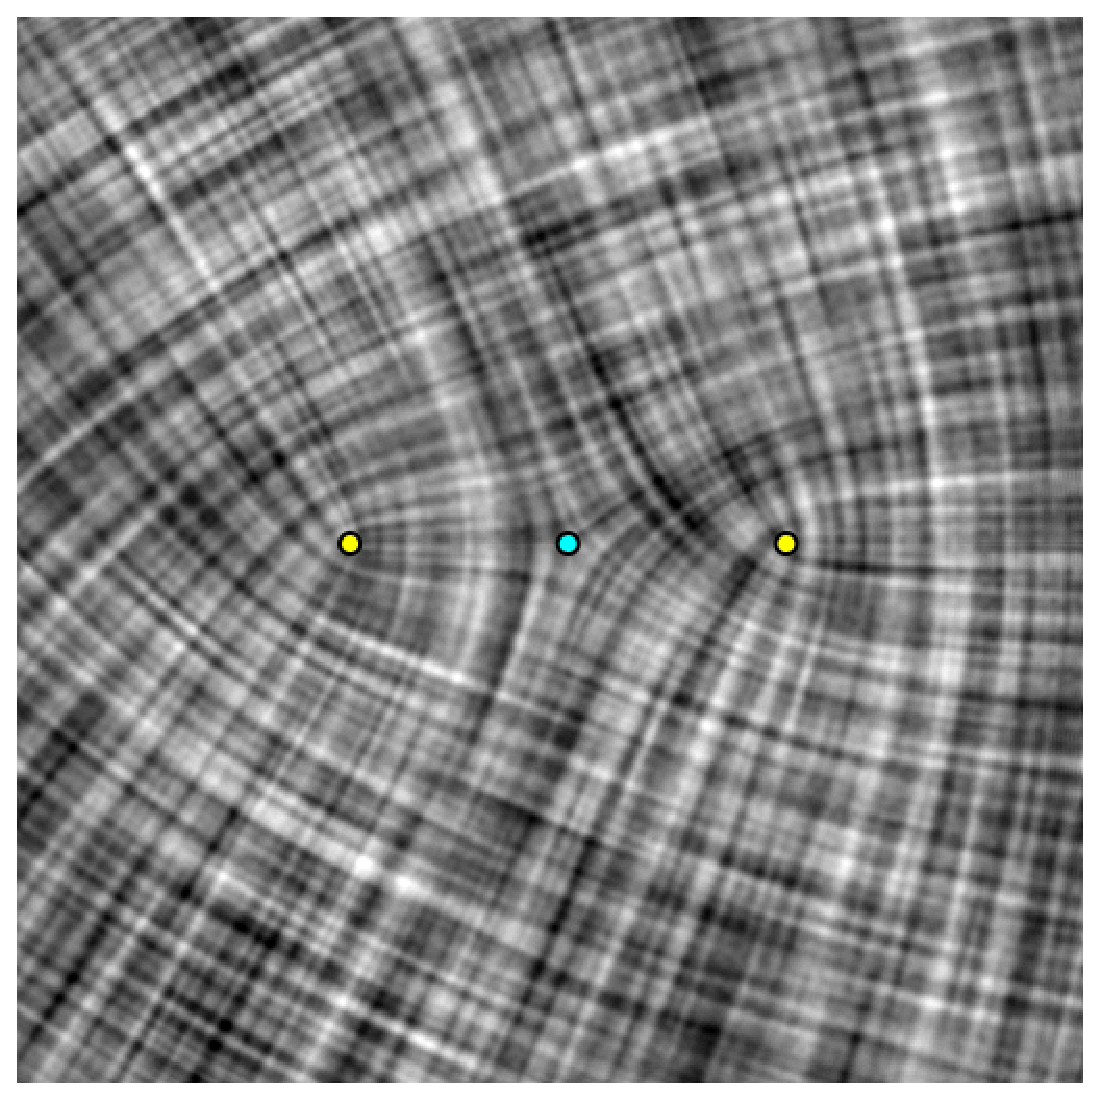
\includegraphics[height=1.07in]{images/cancel_step0_4sym.eps}
    &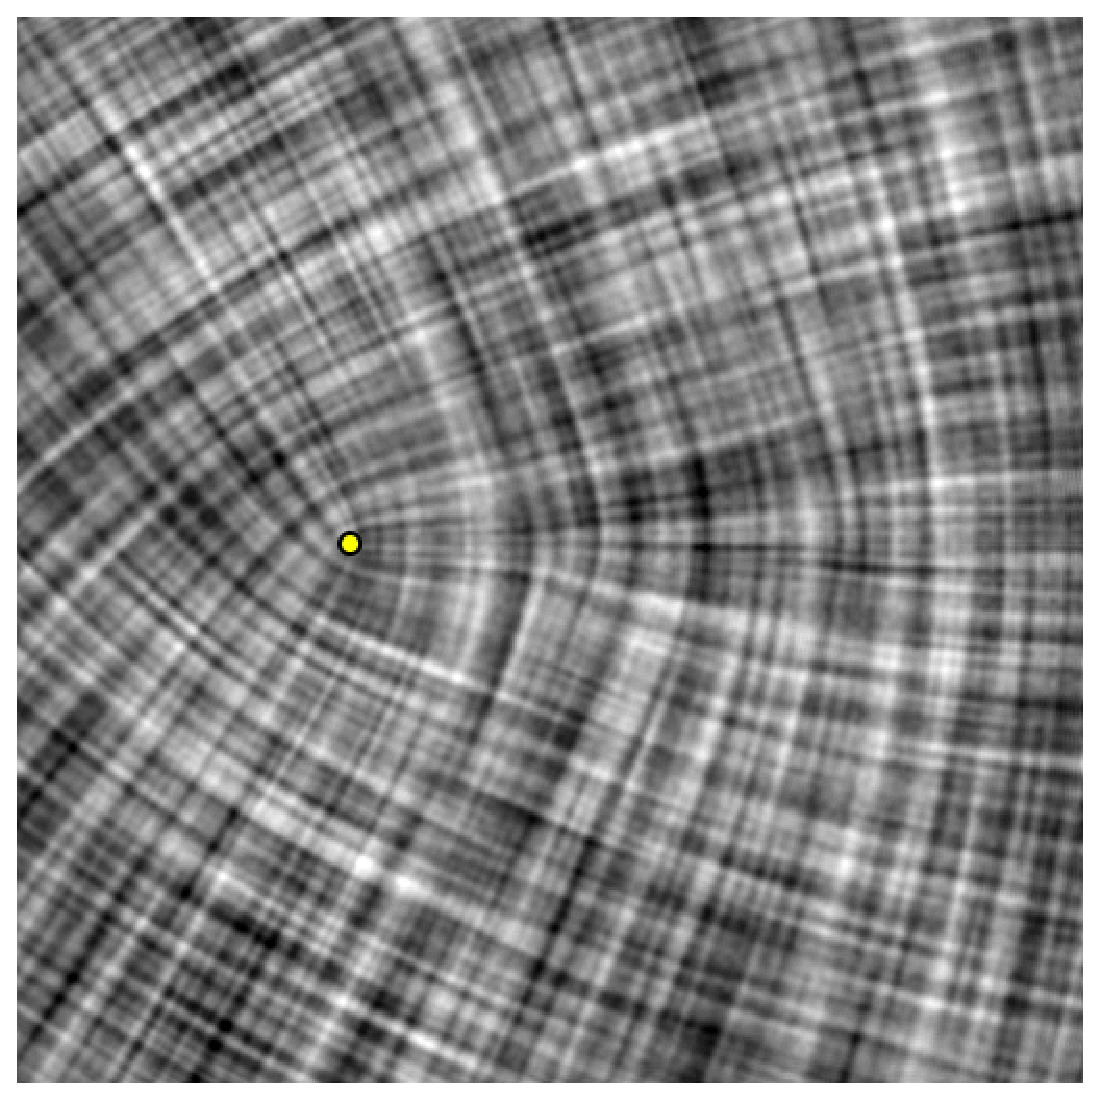
\includegraphics[height=1.07in]{images/cancel_step1_4sym.eps}
    &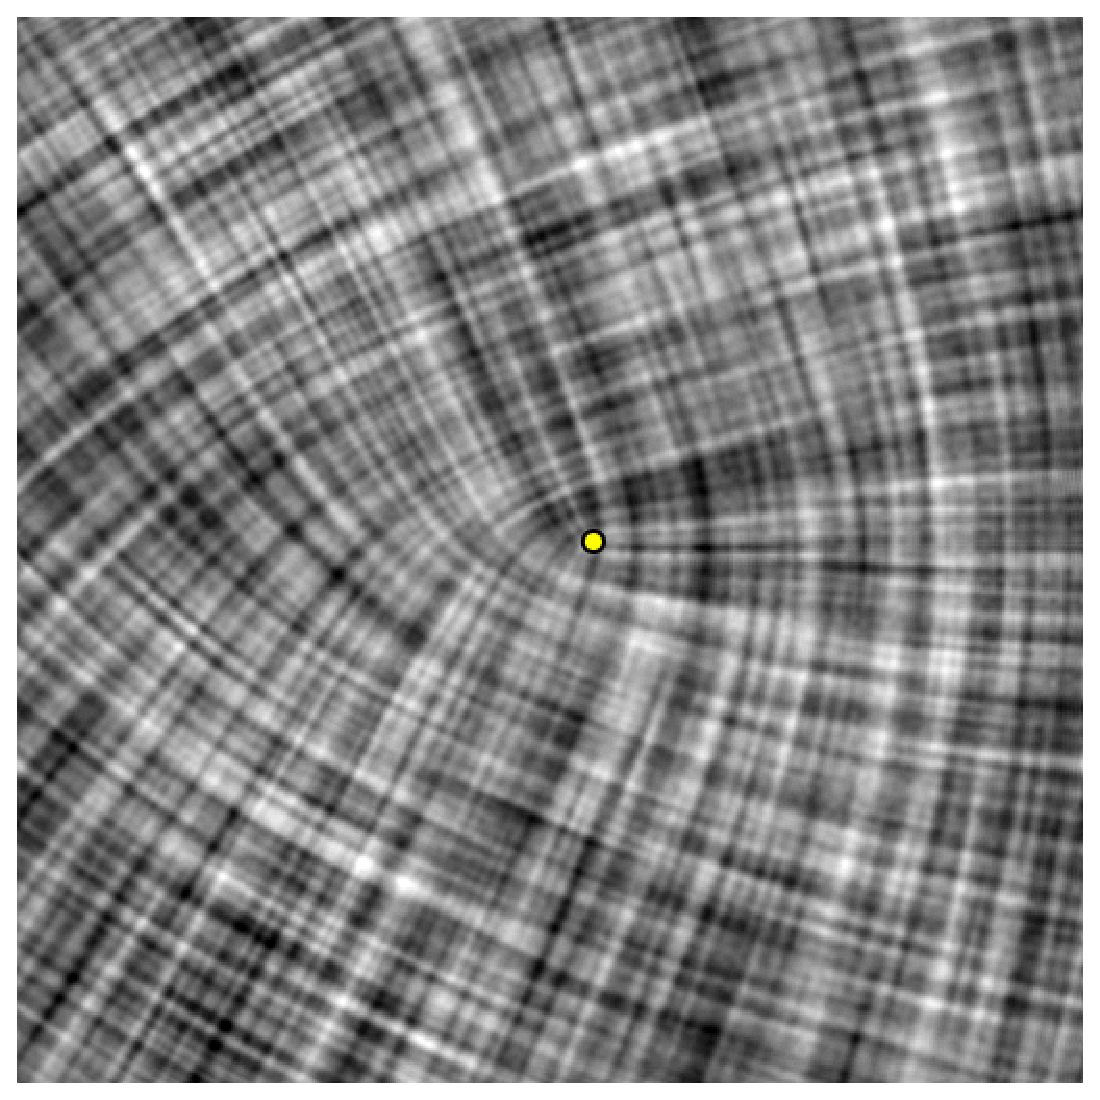
\includegraphics[height=1.07in]{images/cancel_step2_4sym.eps}
    \\
    \end{array}$
\end{center}
\caption{ This figure illustrates the topological editing operations
of our system. The fields shown in the images are: a $4$-Rosy field
with three singularities (left), after singularity pair cancellation
(middle), and after singularity movement (right). The actual editing
was performed on the representation vector fields, which allows us
to reuse corresponding vector field editing operations. }
\label{fig:symmetry_editing}
\end{figure}

Performing singularity pair cancellation and movement on surfaces
requires the ability to conduct Laplacian smoothing on the
representational vector field inside a region. To avoid the use of
surface parameterization that is computationally expensive, we reuse
the idea of parallel transport discussed in
Section~\ref{sec:initialization}, which allows relaxation to be
carried out on surfaces.

\section{Applications}
\label{sec:application}

We have applied our design system to pen-and-ink sketching and
quad-dominant remeshing.

\begin{figure*}[t]
%\centerline{\epsfig{file=images/bimba.eps,angle=0,width=\textwidth}}
\begin{center}
    $\begin{array}{@{\hspace{0.0in}}c@{\hspace{0.05in}}c@{\hspace{0.05in}}c}
    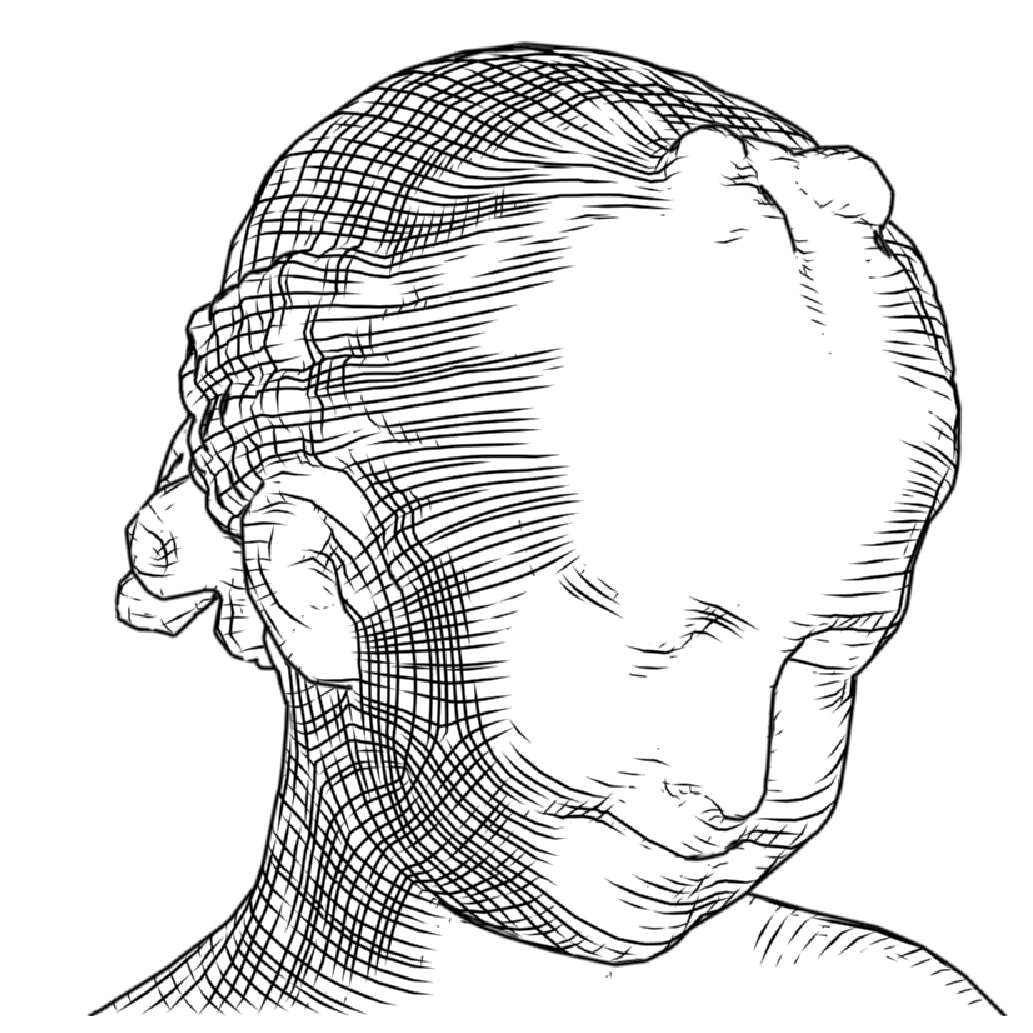
\includegraphics[width=2.3in]{images/bimba_before_antiA.eps}
    &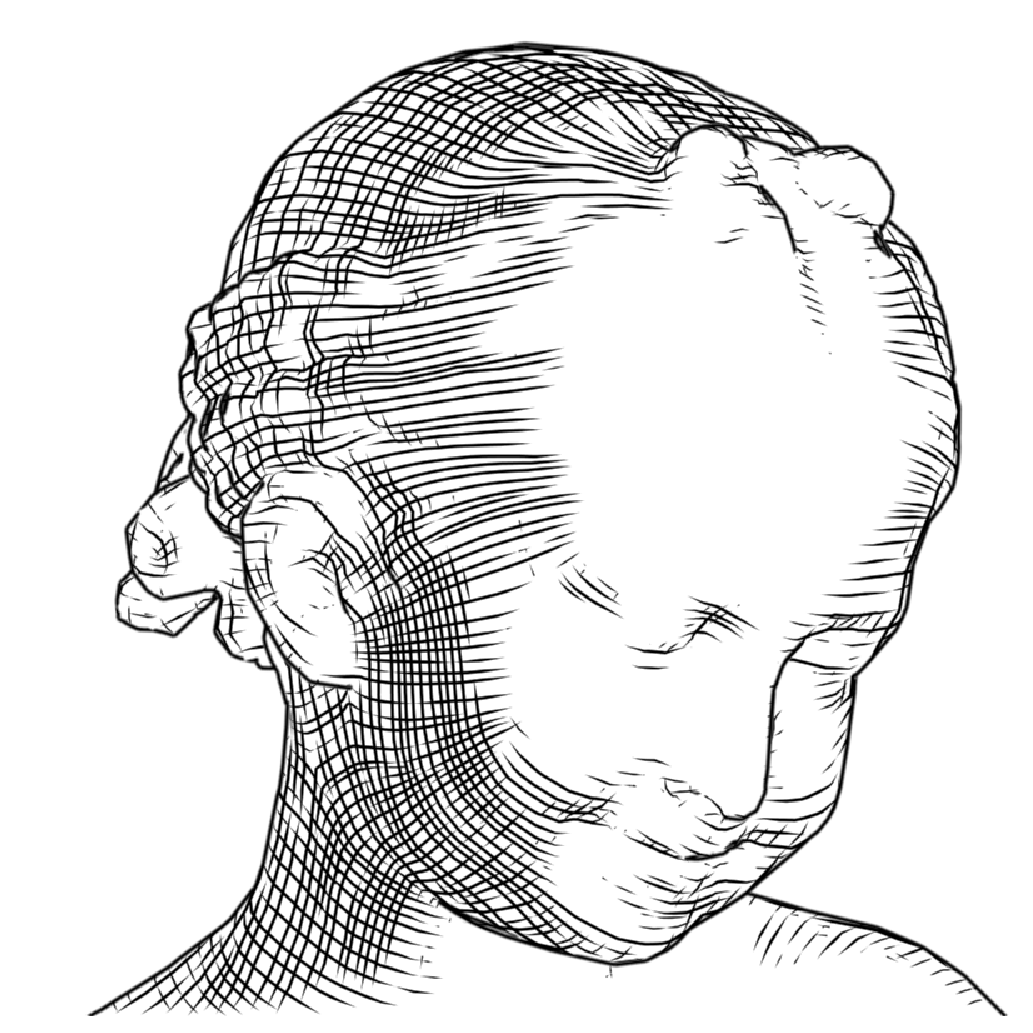
\includegraphics[width=2.3in]{images/bimba_middle_antiA.eps}
    &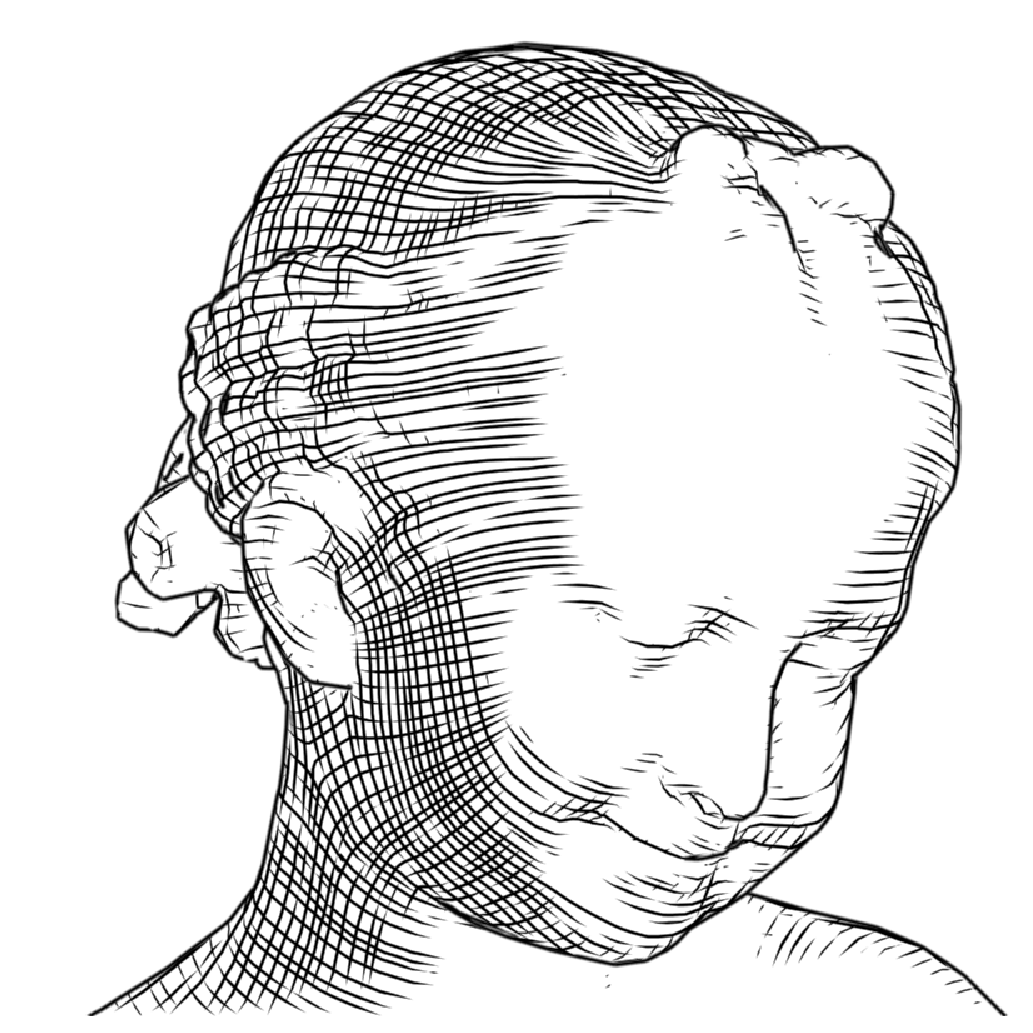
\includegraphics[width=2.3in]{images/bimba_after_antiA.eps}
    \\
%    \includegraphics[width=2.3in]{images/bimba_before.eps}
%    &\includegraphics[width=2.3in]{images/bimba_middle.eps}
%    &\includegraphics[width=2.3in]{images/bimba_after.eps}
%    \\
\end{array}$
\end{center}
\caption{ Topological editing operations were applied to pen-and-ink
sketching of the Bimba model in order to remove visual artifacts
caused by undesirable singularities. The original $4$-RoSy field
(left) contains a number of such singularities on the visible side
of the face (left). Two of them (on the lower side of the face near
the neck) were removed through singularity pair cancellation
(middle). Next, a singularity near the corner of the right eye was
moved to reduce the amount of discontinuity in the hatching
directions near the eye. } \label{fig:result_pen_ink}
\end{figure*}

\subsection{Pen-and-ink Sketching of Surfaces}
\label{sec:pen_and_ink}

Pen-and-ink sketching of surfaces is a non-photorealistic style of
shape visualization. The efficiency of the visualization as well as
the artistic appearance depend on a number of factors, one of which
is the direction of hatches. Girshick et al.~\shortcite{Girshick:00}
show that 3D shapes are best illustrated if hatches follow principle
curvature directions. However, curvature estimation on discrete
surfaces is a challenging problem. While there have been several
algorithms that are theoretically sound and produce high-quality
results~\cite{Hertzmann:00,Meyer:02,Cohen:03,Rusinkiewicz:04}, most
of them still rely on smoothing to reduce the noise in the curvature
estimate. Consequently, these methods do not provide control over
the singularities in the field. Hertzmann and
Zorin~\shortcite{Hertzmann:00} propose the concept of cross fields,
which are $4$-RoSy fields obtained from the curvature tensor (a
$2$-RoSy field) by removing the distinction between the major and
minor principle directions. They demonstrate that smoothing on the
cross field tends to produce more natural hatch directions than
smoothing directly on the curvature tensor. They also point out the
need to control the number and location of the singularities in the
field. Zhang et al.~\shortcite{Zhang:07} address this issue by
providing singularity pair cancellation and movement operations on
the curvature tensor field. However, their technique cannot handle a
$4$-RoSy field.

In this paper, we follow Hertzmann and
Zorin~\shortcite{Hertzmann:00} by treating hatch directions as a
$4$-RoSy field and use topological editing operations to control the
number and location of the singularities.
Figure~\ref{fig:result_pen_ink} illustrates the utility of
topological editing operations with the Bimba model. The original
$4$-RoSy field (left) was obtained from the curvature tensor, which
we computed using the algorithm of Meyer et
al.~\shortcite{Meyer:02}. This field contains three singularities on
the visible side of the face, which cause visual artifacts in the
result. Two of them (on the lower side of the face near the neck)
were removed through singularity pair cancellation (middle), and the
third one (near the corner of the right eye) was moved within the
highlight region (right).

Figure~\ref{fig:teaser} provides the following comparisons with the
Venus model: $2$-RoSy (a) versus $4$-RoSy (b), and topological
editing (c) versus global smoothing (d). Representing the curvature
tensor as a $4$-RoSy field leads to smoother results. Notice the
visual artifacts caused by the singularities on the chest in (a).
The hatch directions in those regions are more natural with
$4$-RoSy's (b). In (c) and (d), we compare topological editing and
global smoothing that can both be used to further reduce the visual
artifacts caused by unwanted singularities. Compare these images to
(b) near the chest and under the armpit. Furthermore, topological
editing operations provide local control that is lacking in global
smoothing. Notice that excessive global smoothing can lead to
significant deviations in the hatch directions. Compare (b) and (d)
around the neck and on the chest. Topological editing operations, on
the other hand, preserve curvature directions in regions where
topological editing was not performed. See the same regions in (c).

%illustrates this with an illustrations of Venus. The field in the
%left is the $4$-RoSy field obtained from the curvature tensor (we
%use the algorithms of Meyer et al.~\shortcite{Meyer:02} to estimate
%the curvature). Notice it contains a number of unwanted or misplaced
%singularities, such as the positive first-order point near the tip
%of the right shoulder, and the negative first-order points in the
%middle of the right shoulder and on the waist. The middle image was
%obtained by performing global smoothing on this field. While the
%visual artifacts of singularities were reduced, hatch directions on
%the right no longer follow the curvature directions. In contrast,
%the field in the right were obtained from the one in the left by
%performing three singularity movement and one pair cancellation
%operations. Notice that visual artifacts of the singularities were
%reduced, and hatch directions still follow curvature directions on
%the right shoulder and along the waist.

\begin{figure}[t]
\begin{center}
    $\begin{array}{@{\hspace{-0.02in}}c@{\hspace{0.0in}}c}
%    \includegraphics[width=1.7in]{images/bunny_remesh_before_fld.eps}
%    &\includegraphics[width=1.7in]{images/bunny_remesh_before.eps}\\
%    (a) & (b) \\
    \includegraphics[width=1.7in]{images/bunny_remesh_too_smooth_fld.eps}
    &\includegraphics[width=1.7in]{images/bunny_remesh_too_smooth.eps}\\
%    (c) & (d) \\
    \includegraphics[width=1.7in]{images/bunny_remesh_after_fld.eps}
    &\includegraphics[width=1.7in]{images/bunny_remesh_after.eps}\\
%    (e) & (f) \\
\end{array}$
\end{center}
\caption{ $4$-RoSy field design was applied to quad-dominant
remeshing. The field in the top was obtained by performing smoothing
on a $4$-RoSy field derived from the curvature tensor, while the
field in the bottom was obtained by performing a sequence of
topological editing operations on the same tensor field. Notice that
while both fields are smooth, the field in the bottom contains
singularities that situate in natural locations such as near the
leg. In contrast, the field in the top is overly smooth and does not
follow the curvature directions in many parts of the model. }
\label{fig:quad_remesh}
\end{figure}

\subsection{Quad-Dominant Remeshing}
\label{sec:remeshing}

The problem of quad-dominant remeshing, i.e., constructing a
quad-dominant mesh from an input mesh, has been a well-studied
problem in computer graphics. The key observation is that a nice
quad-mesh can be generated if the orientations of the mesh elements
follow the principle curvature directions~\cite{Alliez:03}. This
observation has led to a number of efficient remeshing algorithms
that are based on streamline
tracing~\cite{Alliez:03,Marinov:04,Dong:05}. Ray et
al.~\shortcite{Ray:06} note that better meshes can be generated if
the elements are guided by a $4$-RoSy field. They also develop an
energy functional that can be used to generate a periodic global
parameterization and to perform quad-based remeshing. The connection
between quad-dominant remeshing and $4$-Rosy fields has also
inspired Tong et al.~\shortcite{Tong:06} to generate quad meshes by
letting the user design a {\em singularity graph} that resembles the
behavior of the topological skeleton of a $4$-RoSy field. On the
other hand, Dong et al.~\shortcite{Dong:06} perform quad-remeshing
using spectral analysis, which produces quad meshes that in general
do not align with the curvature directions.

We apply our design system to a $4$-RoSy field that is obtained from
principle curvature directions by not distinguishing between the
major and minor directions. Our method is based on streamline
tracing. In contrast to most existing approaches, we first trace all
the separatrices for a certain distance. This allows singularities
to be the vertices in the new mesh and that the nearby regions
consist of nice quad elements (Figure~\ref{fig:quad_remesh}). Notice
that this would not have been possible without the analysis of
$N$-RoSy fields. In addition, $4$-RoSy field design enhances the
chance of obtaining a better mesh by removing noise and placing
singularities in natural locations. Figure~\ref{fig:quad_remesh}
illustrates this with two examples fields, both were obtained by
editing a $4$-RoSy field corresponding to the curvature tensor. The
top field corresponds to a sequence of global smoothing, which tends
to lose sharp features in the model and no longer follows the
principle curvature directions. The bottom field, on the other hand,
was obtained through a sequence of singularity editing operations
that allow singularities to be edited in an isolated fashion, thus
maintain sharp features and natural singularities.

We wish to emphasize that the focus of our work is on the analysis
and design of $N$-RoSy fields. While we have employed a
streamline-based remeshing approach~\cite{Alliez:03} to demonstrate
the capabilities of our system, fields designed using our system can
potentially be input to other and more recent remeshing techniques
such as~\cite{Ray:06}.

\begin{figure}[t]
\centerline{\epsfig{file=images/dragon_hiRes.eps,angle=0,width=3.0in}}
%\centerline{\epsfig{file=images/dragon_hiRes_thick.eps,angle=0,width=\columnwidth}}
\caption[]{ A $6$-RoSy field designed using our system. Notice that
the network of streamlines resembles a highly regular triangulation.
}\label{fig:triangle}
\end{figure}

\section{Conclusion}
\label{sec:conclusion}

In this paper, we have developed a design system for $N$-RoSy fields
on surfaces with explicit control over the number and location of
singularities in the fields. We demonstrate the effectiveness of our
system with applications in non-photorealistic rendering and
quad-dominant remeshing.

As part of our system, we describe a mathematically sound
representation for $N$-RoSy's that is based on higher-order
symmetric tensors. This link allows us to define algebraic
operations as well as analytic characteristics such as
singularities, differentiability, and continuity. Furthermore, we
present a compact vector-based representation of $N$-RoSy fields on
mesh surfaces that makes it possible to perform field smoothing
using linear systems.

We also provide topological analysis of $N$-RoSy fields and
efficient algorithms with which singularities and separatrices can
be identified.
%We also
%present a framework for the visualization of $N$-RoSy fields that is
%fast and high quality when $N$ is small, such as $2$, $3$, $4$, and
%$6$.

In the future, we plan to investigate the use of $6$-RoSy field
design to obtain optimal triangulations from an input mesh.
Figure~\ref{fig:triangle} demonstrates this potential with a
user-guided $6$-RoSy field on the dragon. Notice that the
streamlines according to field, while not aligned perfectly,
intersect at angles that are multiples of $\frac{\pi}{6}$.
Adaptation of quadrangulation methods such as~\cite{Ray:06,Tong:06}
has the potential of generating high-quality triangular meshes.

In many applications, multiple, coexisting symmetries of different
$N$'s are of interest, such as pen-and-ink sketching and texture
synthesis. We plan to investigate a mathematical framework with
which such objects can be analyzed and designed.

\section*{Appendix: $N$-RoSy's and $N$-th Order Tensors}
\label{sec:higher_tensors}

In this appendix, we point out the link between $N$-RoSy's and
$N$-th order covariant symmetric tensors, which justifies the way in
which the components of a representation vector transform under a
change of basis (Section~\ref{sec:representation}).

Recall that when $N=1$ and $2$, an $N$-RoSy can be modeled as a
vector or a symmetric traceless matrix~\cite{Zhang:07},
respectively. When $N \ge 3$, we turn to $N$-th order tensors and
define an injective map $\alpha$ from the set of two-dimensional
$N$-RoSy's into the set of two-dimensional $N$-th order symmetric
tensors. $\alpha$ allows algebraic operations on $N$-RoSy's to be
defined in terms of corresponding operations on $N$-th order
tensors. Before describing $\alpha$, we briefly review relevant
facts about $N$-th order tensors. Given an othonormal basis for
$\mathbb{R}^2$, an $N$-th order covariant {\em tensor} $t=t_{i_1 ...
i_N}$ ($1 \le i_1, ..., i_N \le 2$) is a multi-linear form

\begin{equation}
t(w_1, ..., w_N)=t_{i_1 ... i_N}w_1^{i_1}  ...  w_N^{i_N}
\end{equation}

\noindent where $w_j$'s ($1\le j \le N$) are two-dimensional vectors
and $w_k^{i_k}$ refers to the $i_k$-th component of $w_k$. Here we
are using the {\em Einstein convention} in which the summation signs
are omitted. $t$ is {\em symmetric} if $t_{i_1 ... i_N}=t_{i_{p(1)}
... i_{p(N)}}$ for any permutation $p$ over the set $\{1, ..., N\}$.
In the remainder of the discussion we will only focus on covariant
and symmetric tensors and therefore omit the words {\em symmetric}
and {\em covariant} for convenience.

Given an $N$-RoSy

\begin{equation}
s = \{R\begin{pmatrix} \cos(\theta + \frac{2k\pi}{N}) \\ \sin(\theta
+ \frac{2k\pi}{N}) \end{pmatrix} \mid 0 \le k \le N-1 \}
\end{equation}

\noindent we consider the following $N$-th order tensor
%
%
%In order to define $\alpha$, the map from $N$-RoSy's to $N$-th order
%tensors, we re-examine the relationship between a traceless
%symmetric matrix and its eigenvectors. A $2 \times 2$ symmetric
%traceless matrix $t$ has the following form~\cite{Zhang:07}:
%$R\begin{pmatrix} \cos2\theta & \quad \sin2\theta \\ \sin2\theta &
%-\cos2\theta
%\end{pmatrix}$ where $R$ and $\theta$ represent the strength and
%direction of anisotropy in the tensor, respectively. The major and
%minor eigenvectors are $\mu
%\begin{pmatrix} \cos\theta & \sin\theta
%\end{pmatrix}^{\bf T}$ and
%$\mu \begin{pmatrix} \cos(\theta+\frac{\pi}{2}) &
%\sin(\theta+\frac{\pi}{2}) \end{pmatrix}^{\bf T}$ ($\mu \ne 0$),
%respectively. Furthermore, $t(w, w)=t_{i_1 i_2}w^{i_1} w^{i_2} =
%R\cos2(\theta-\phi)$ where $w = \begin{pmatrix} \cos\phi & \sin\phi
%\end{pmatrix}^{\bf T}$ is a unit vector. In particular, $t(w, w)$ achieves
%its maximum $R$ when $w$ is a major eigenvector and its minimum $-R$
%when $w$ is a minor eigenvector. To extend the above relationship to
%$N \ge 3$, we consider the following $N$-th order tensor $t$:

\begin{equation}
t_{i_1 ... i_N} = \left\{ \begin{array}{ll} \quad R\cos(N\theta) & \textrm{ if $i_1+i_2+..+i_N \equiv 0 \mod 4$} \\
\quad R\sin(N\theta) & \textrm{ if $i_1+i_2+..+i_N \equiv 1 \mod 4$}
\\ -R\cos(N\theta) & \textrm{ if $i_1+i_2+..+i_N \equiv 2 \mod 4$} \\
-R\sin(N\theta) & \textrm{ if $i_1+i_2+..+i_N \equiv 3 \mod 4$}
\end{array} \right.  \label{eq:higherorder_tensor}
\end{equation}.

Given a vector $w=\begin{pmatrix} \cos\phi \\ \sin\phi
\end{pmatrix}$, it is straightforward to verify that $t(w, ..., w) =
R\cos N(\theta-\phi)$. Furthermore, it can be shown that $t$ is the
only tensor that has this property. $t(w, ..., w)$ achieves its
maximum on the unit circle $S^1$ when $\theta - \phi \equiv 0 \mod
\frac{2\pi}{N}$. There are $N$ such vectors, which are exactly the
member vectors of $s$. This allows us to map $s$ to $t=\alpha(s)$ as
defined in Equation~\ref{eq:higherorder_tensor}.
% This definition is consistent when $N=1$ and $2$.
When $N=1$, $s$ is a vector and $t=s$ is also a vector. When $N=2$,
$t$ is the traceless symmetric matrix whose major eigenvalue is $R$
and major eigenvectors are given by the member vectors of $s$.

%Given two $N$-RoSy's $s_1$ and $s_2$ and $\lambda \in \mathbb{R}$,
%we define $s_1+s_2 = \alpha^{-1}(\alpha(s_1)+\alpha(s_2))$ and
%$\lambda s_1 = \alpha^{-1}(\lambda \alpha(s_1))$. These definitions
%allow us to define important concepts on $N$-RoSy fields, such as
%continuity, singularity, and differentiability.

Notice that tensors defined in Equation~\ref{eq:higherorder_tensor}
form a two-dimensional linear subspace of the set of $N$-th order
tensors, which leads to the following construction of a bijective
map $\beta$ from the subspace to a two-dimensional vector space such
that

\begin{equation}
\beta(t_{i_1 ... i_N}) = \begin{pmatrix} t_{0 0 ... 0} \\ t_{1 0 ...
0} \end{pmatrix} = \begin{pmatrix} R\cos N\theta \\ R\sin N\theta
\end{pmatrix}
\end{equation}

The composite map $\gamma = \beta \circ \alpha$ has been used to map
an $N$-RoSy to its representation vector as described in
Section~\ref{sec:representation}. As a compact representation of an
$N$-th order tensor, the components of a representation vector
transform differently than a vector under a change of basis.

\section*{Acknowledgements}

We would like to thank the following people and groups for the 3D
models they provided: Mark Levoy and the Stanford Graphics Group,
Cyberware, and the AIM@SHAPE Shape Repository. The discussions with
Greg Turk have been valuable. We are also grateful for the help of
Patrick Neill and Guoning Chen in preparing the video production.
Finally, we wish to thank our reviewers for their excellent comments
and suggestions. This work is funded by NSF grant CCF-0546881.

%\fontsize{8pt}{8pt}\selectfont
%\itemsep 0.0in
%\parskip 0.03in
%\parsep 2pt


\bibliographystyle{acmsiggraph}
\nocite{*}
\bibliography{symmetry}
\end{document}
